\section{Results}

\subsection{Business as Usual}

This scenario does two things. First, by comparing the electricity generation
over the course of the next 10 years to a reference year, 2014, we can validate
the results from \gls{temoa}. Second, it motivates the need to include other
energy sources.
In Figure \ref{fig:bau-2014}, the \texttt{IMPELC-2014}
and \texttt{TURBINE-2014} bars refer to imported electricity and turbines
at \gls{app} in 2014, respectively.

\begin{figure}[ht]
	\centering
	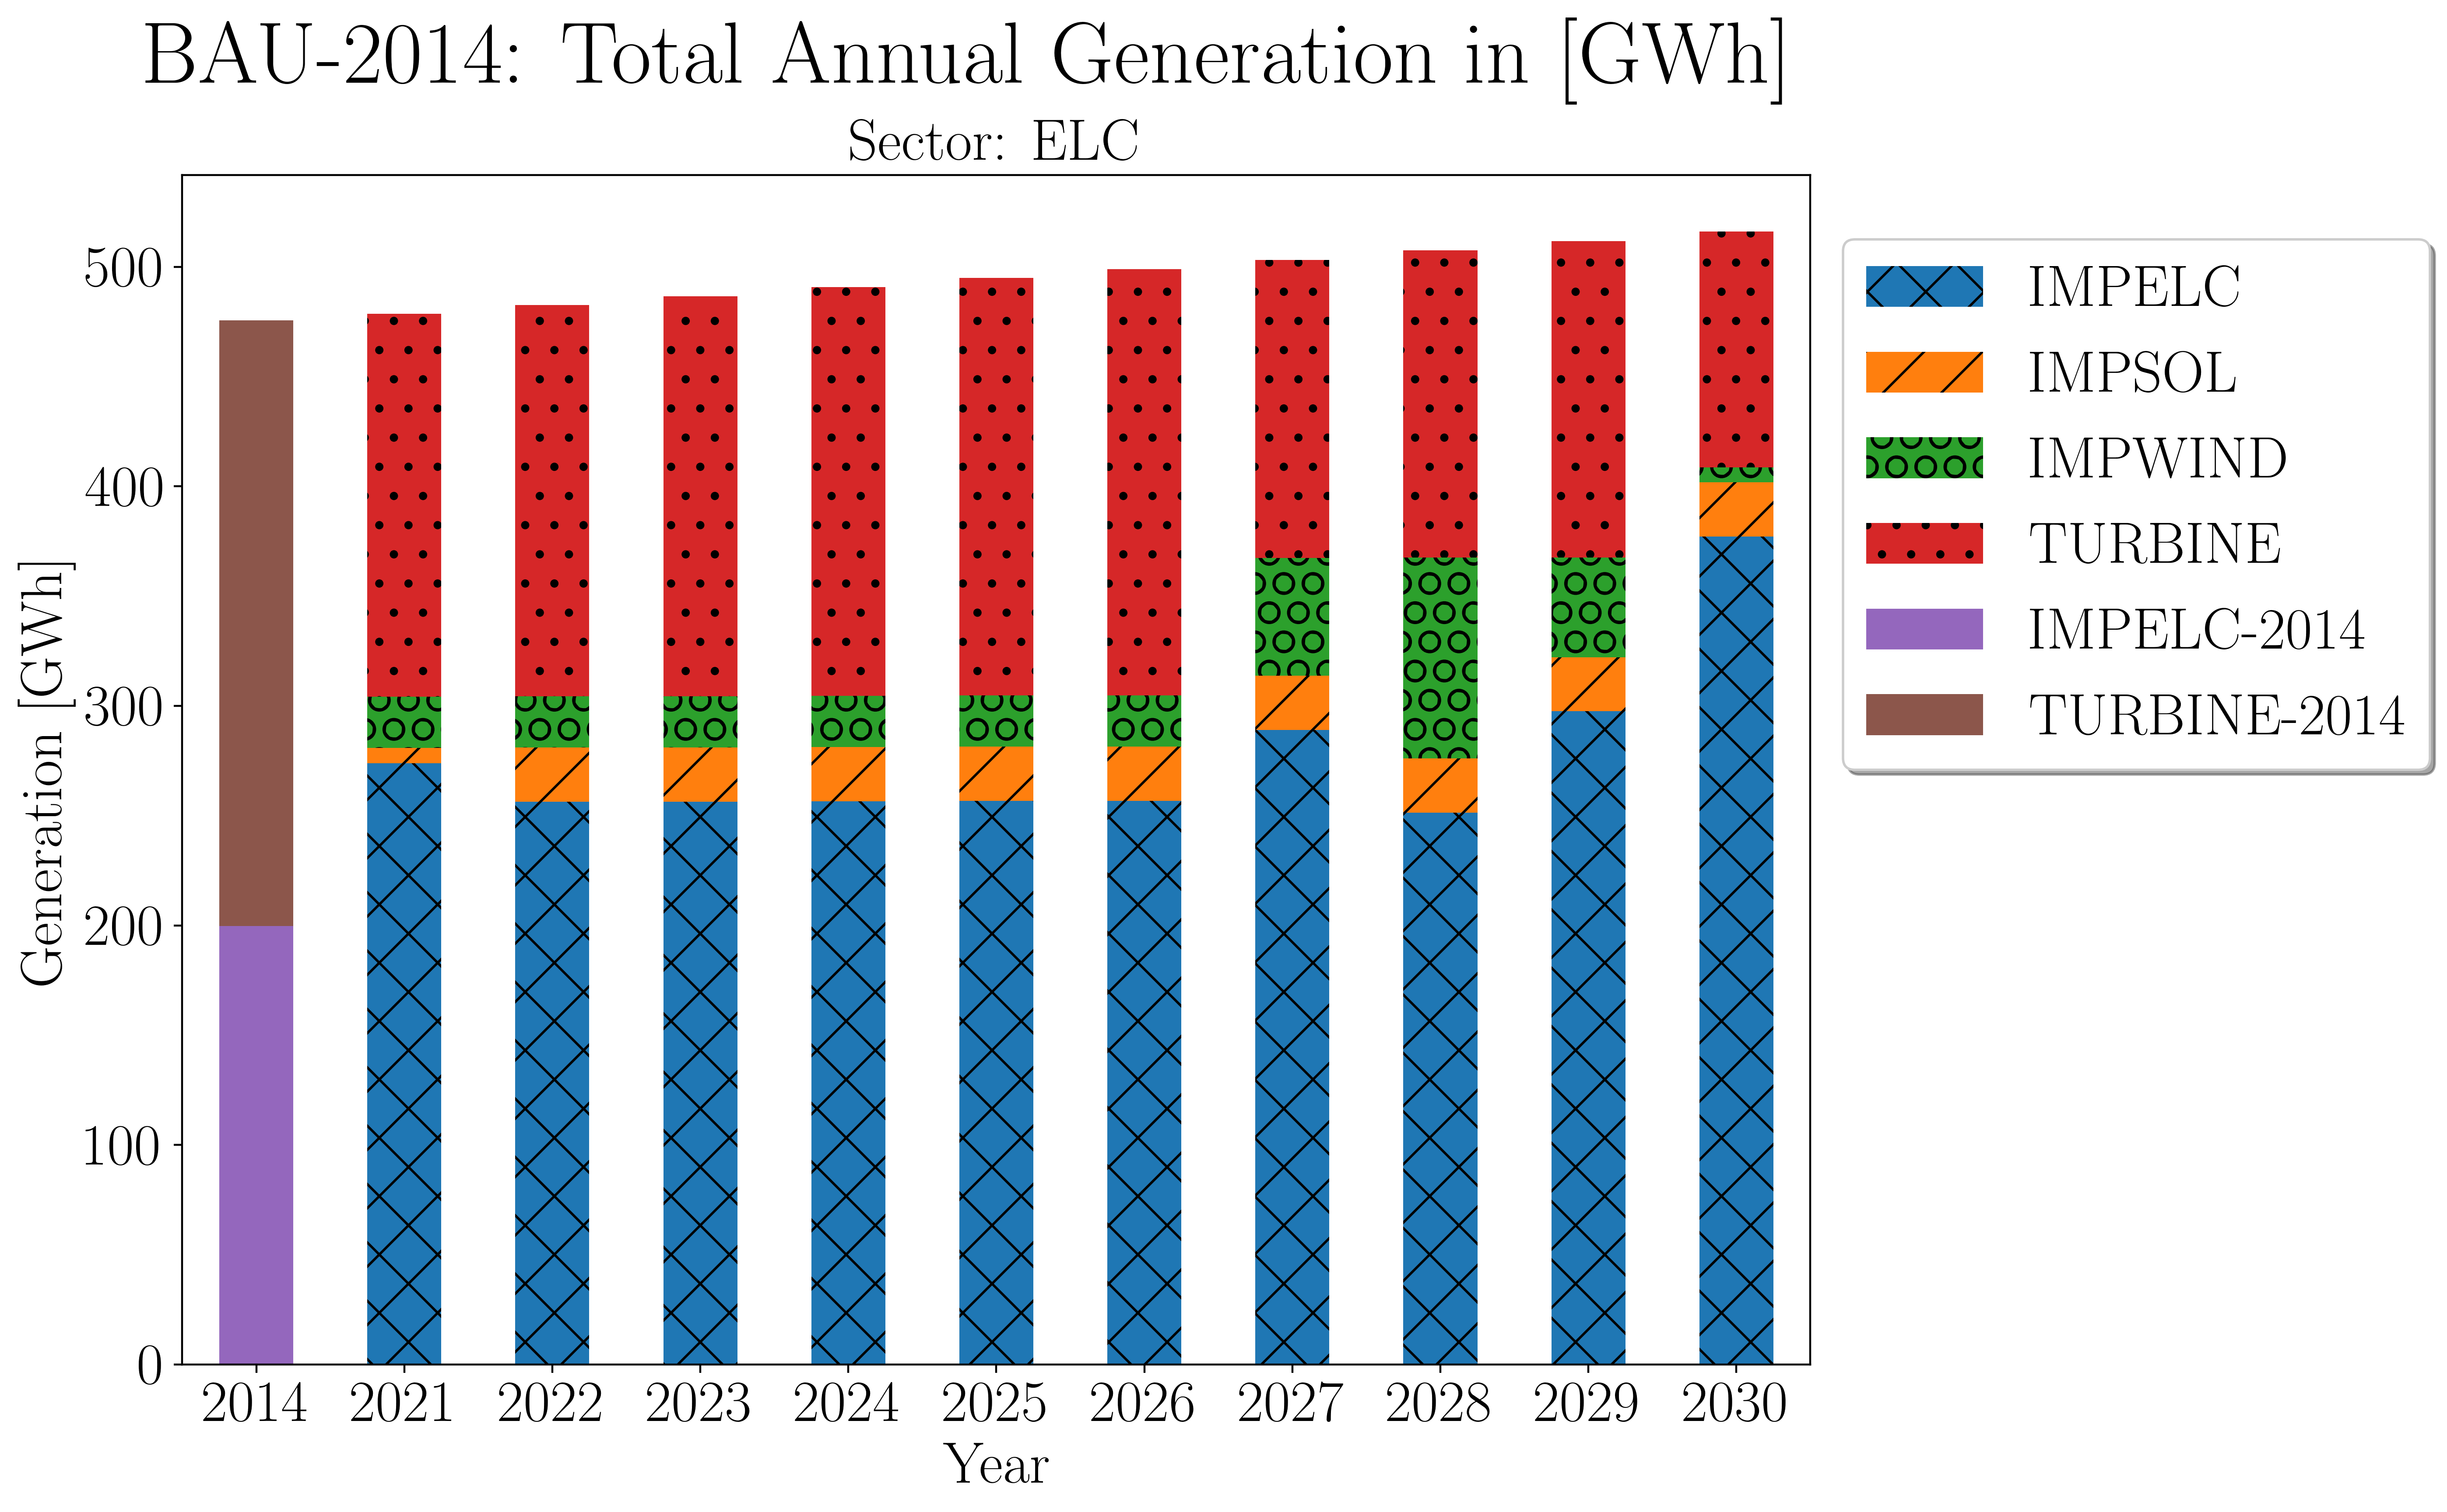
\includegraphics[width=\columnwidth]{BAU-2014_elc_generation.png}
	\caption{The predicted electric generation in GWh(e) for the next 10 years
	from Temoa, compared with data from 2014 \cite{isee_illinois_2015}.}
	\label{fig:bau-2014}
\end{figure}

UIUC had neither a solar farm nor a \gls{ppa} with a wind farm
in 2015 when \gls{icap} was published.
The electricity that those two sources now displace would have been produced by
the natural gas plant, \gls{app}.
The \gls{uiuc} Master Plan \cite{affiliated_engineers_inc_utilities_2015}
also indicates that increasing electricity imports in the near term will be
important for meeting the electricity demands of the university. This
recommendation matches the trend shown in Figure \ref{fig:bau-2014}.
The carbon emissions projected by \gls{temoa} are shown in Figure \ref{fig:bau-emissions}
also match the carbon emissions in the \gls{icap} document
\cite{isee_illinois_2015}, which rises to about 500
ktons of carbon equivalent by 2030. The similarities between the \gls{temoa}
model and \gls{icap} further validates the model results.

\begin{figure}[ht]
	\centering
	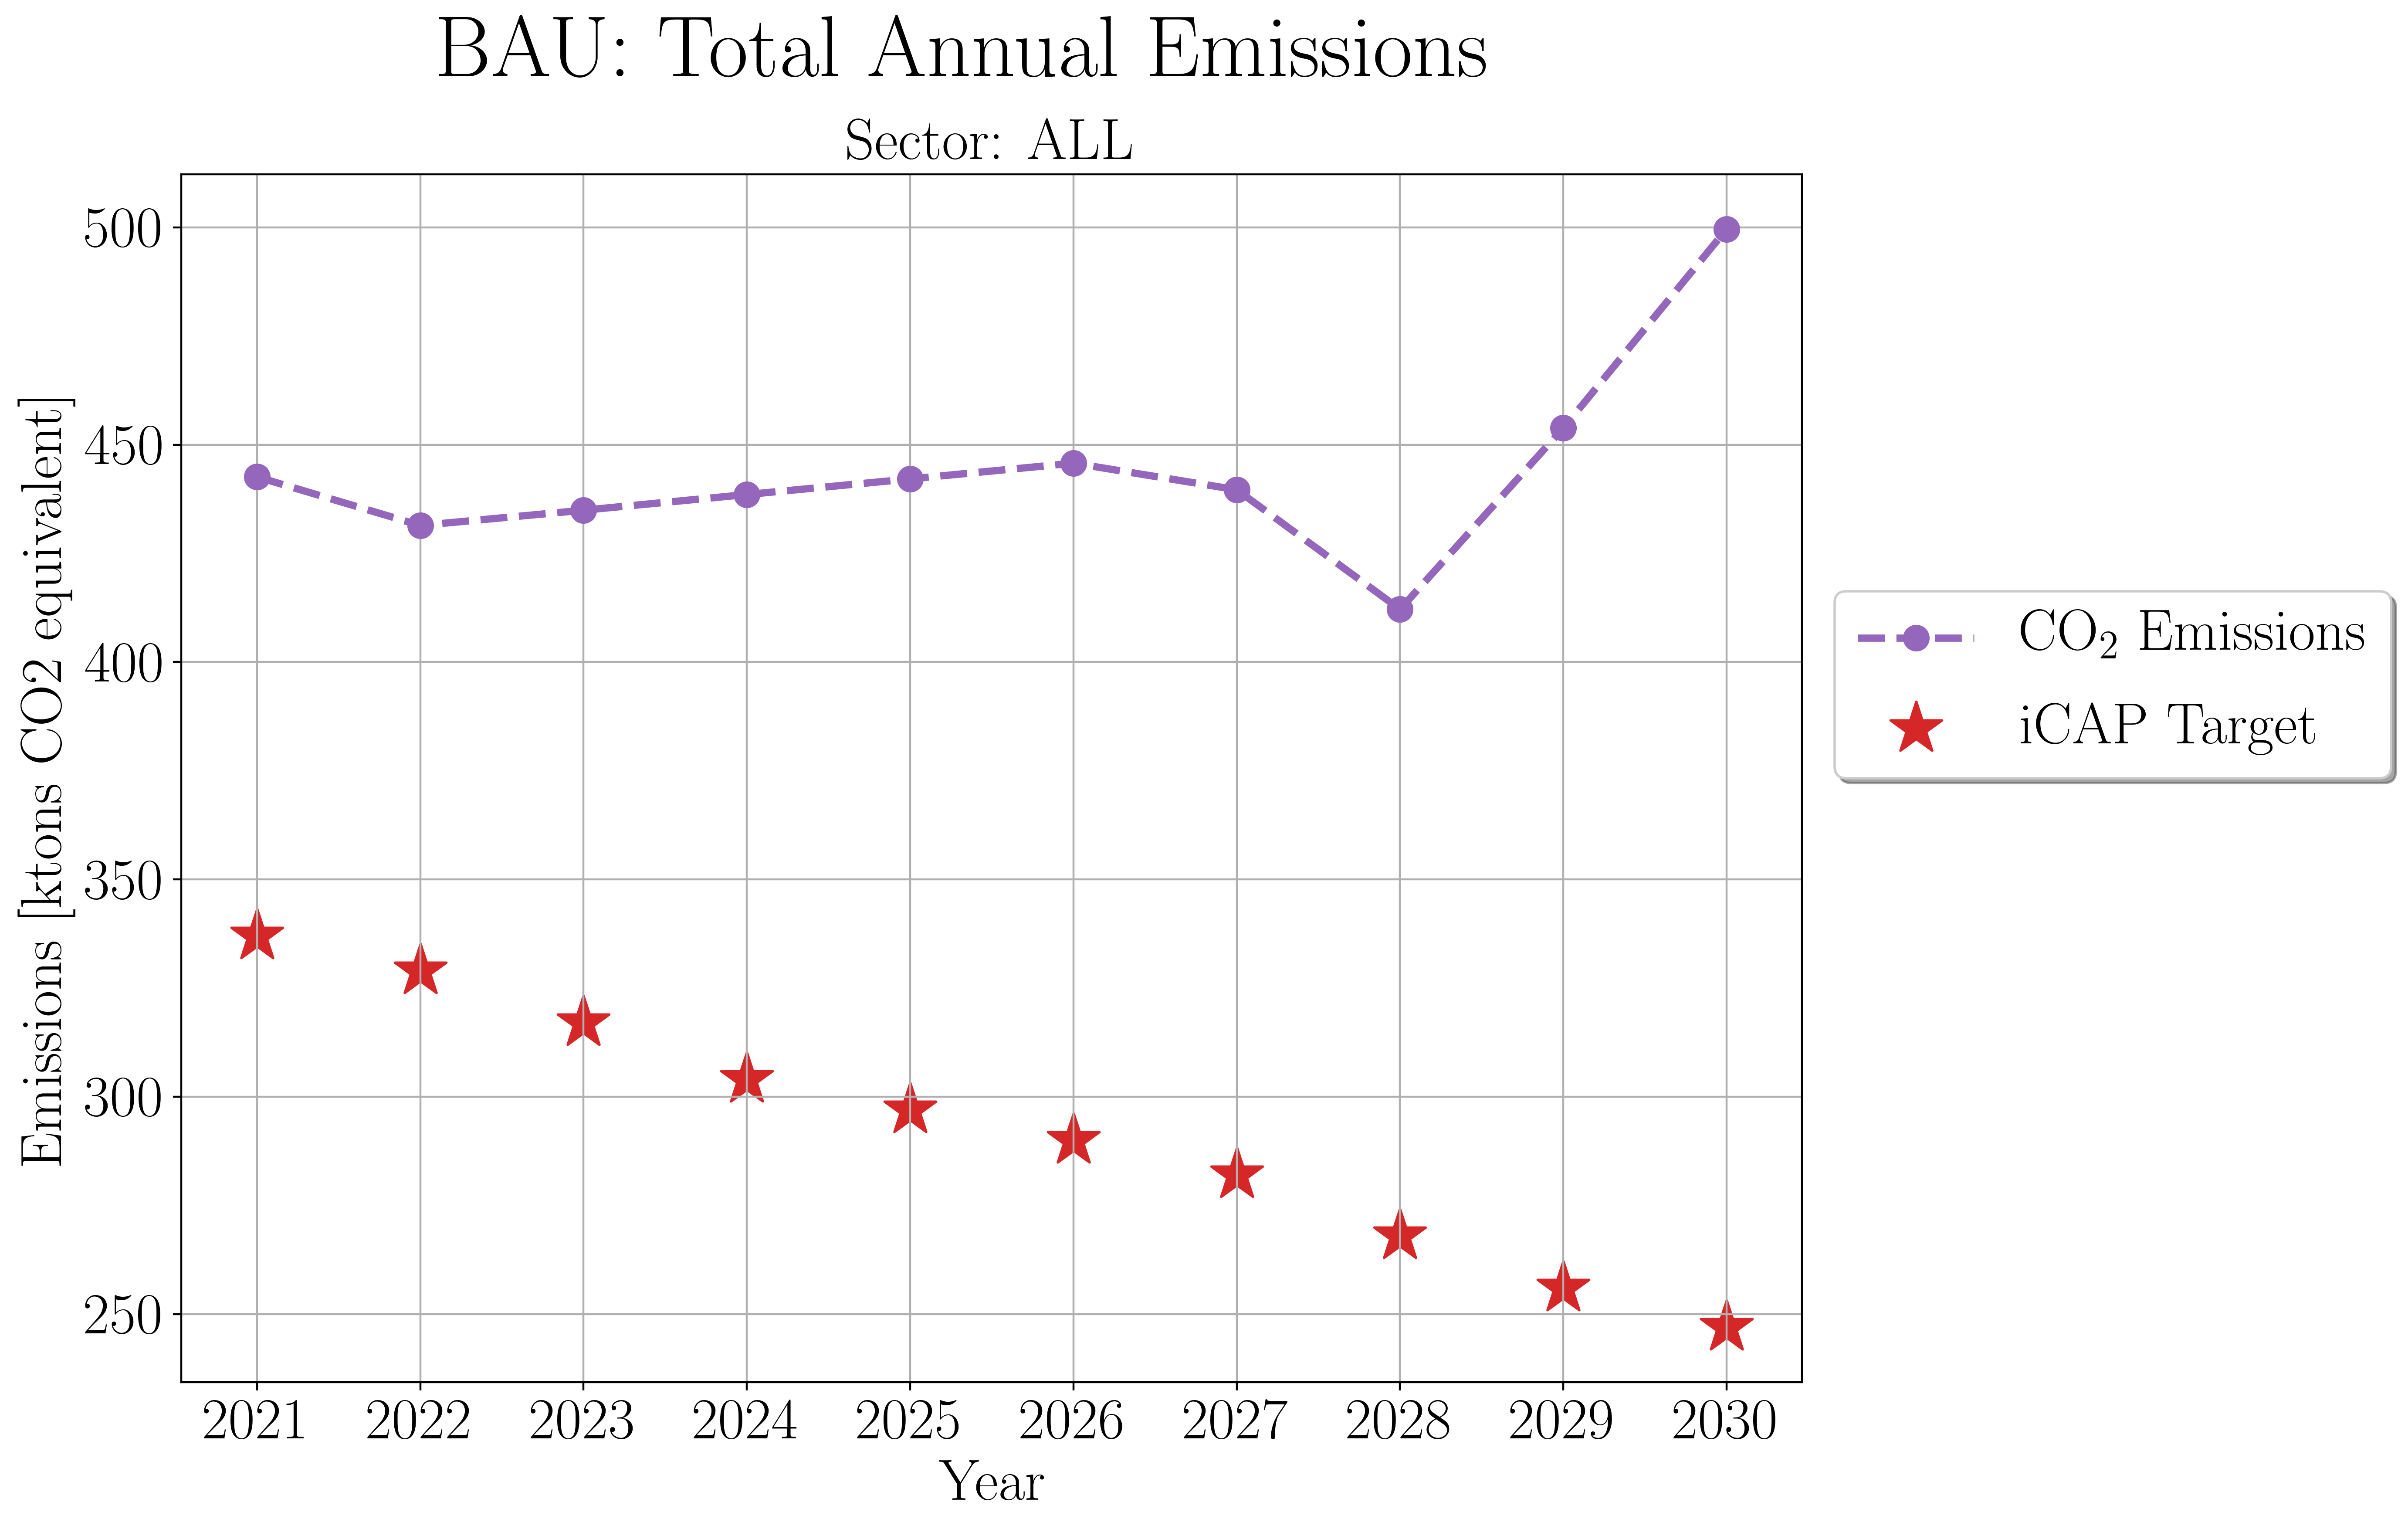
\includegraphics[width=\columnwidth]{bau_all_emissions.png}
	\caption{The Temoa projected carbon emissions for the next 10 years if
	\gls{uiuc} continues with ``business as usual.''}
	\label{fig:bau-emissions}
\end{figure}

Unless \gls{uiuc} halts its growing demand for electricity the University will
not achieve its carbon goals \cite{isee_illinois_2015, affiliated_engineers_inc_utilities_2015}.


\subsection{Scenario 1: Zero Capital Cost Nuclear Reactor}

This scenario shows an idealized solution for reducing carbon
emissions at \gls{uiuc} if nuclear reactors could be built with no capital cost.
For this idealized case, Figure \ref{fig:s01_ind_cap} and \ref{fig:s01_ind_gen}
show that \gls{app} would be immediately replaced by a nuclear reactor. Even
though Figure \ref{fig:s01_ind_cap} shows the nuclear reactor capacity growing
to 2000 MW$_{th}$, Figure \ref{fig:s01_ind_gen} shows that this is
unecessary and the demand for steam and electricity could be satisfied by
a reactor around 375 MW$_{th}$.

\begin{figure}[ht!]
	\centering
	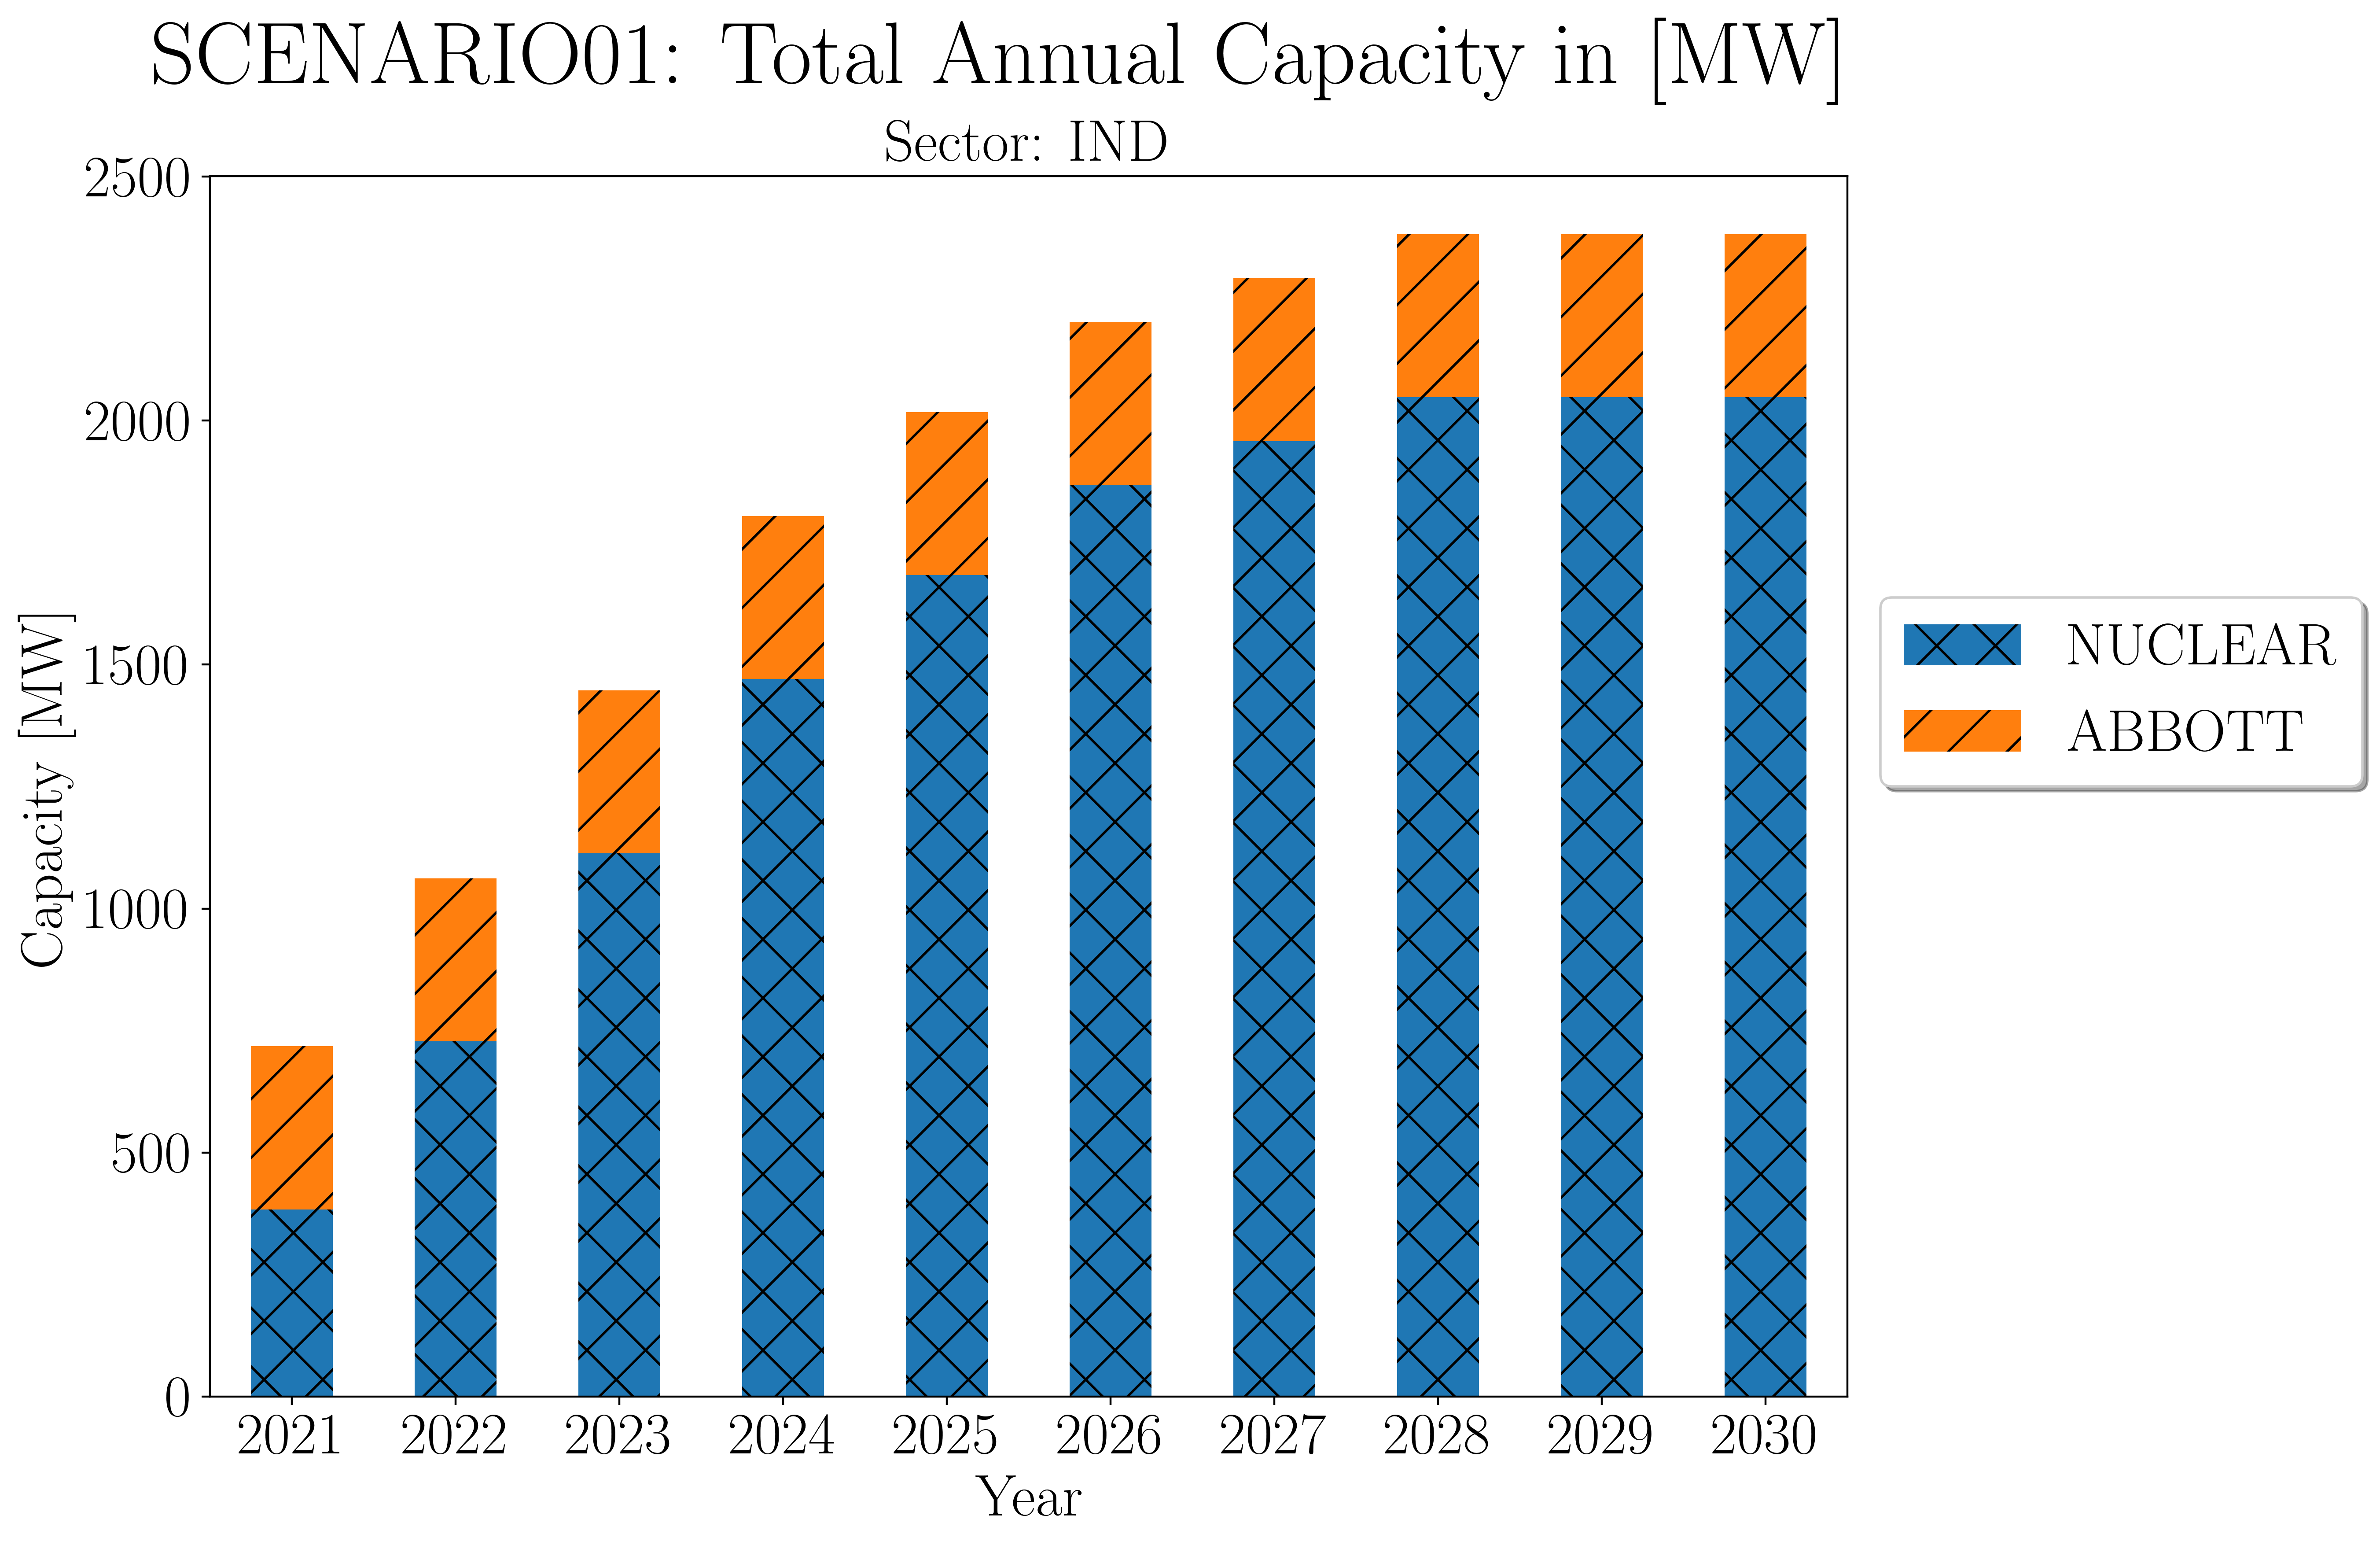
\includegraphics[width=\columnwidth]{scenario01_ind_capacity.png}
	\caption{The projected steam generation in MW$_{th}$ for the next 10 years
	if \gls{uiuc} could build nuclear reactors at no cost.}
	\label{fig:s01_ind_cap}
\end{figure}

\begin{figure}[ht!]
	\centering
	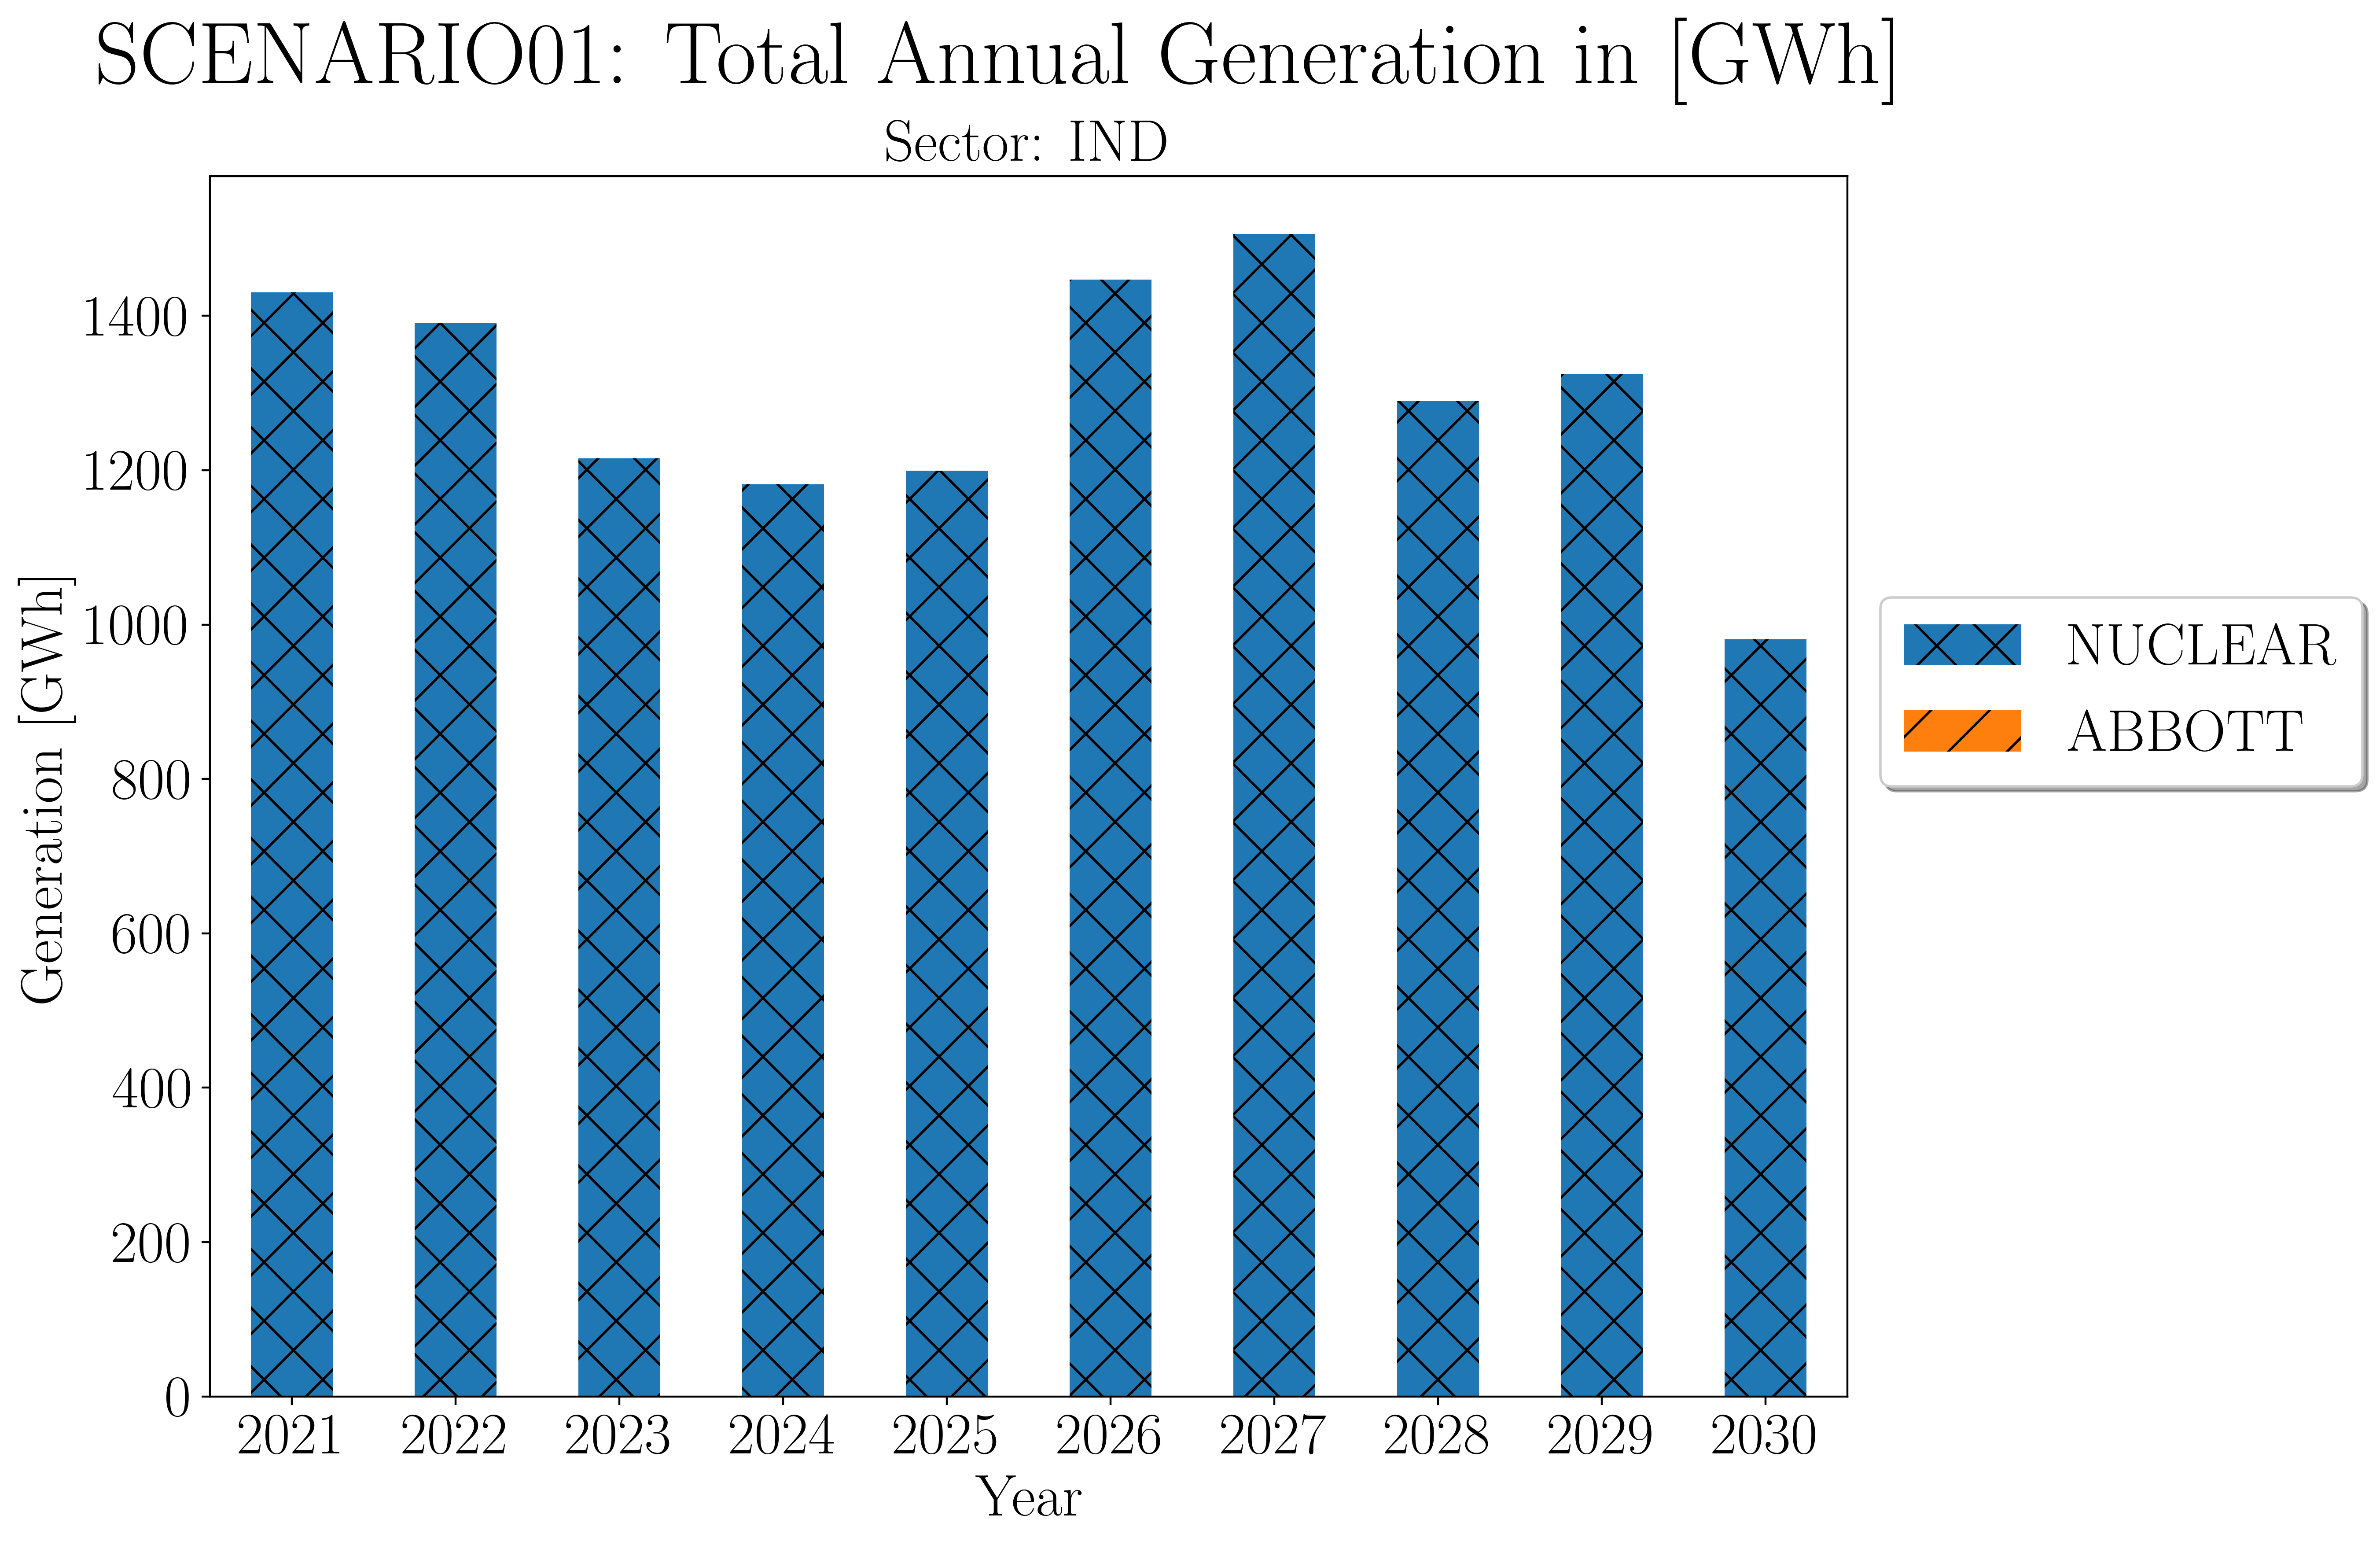
\includegraphics[width=\columnwidth]{scenario01_ind_generation.png}
	\caption{The projected breakdown of steam generation by source in GWh(th)
	for the next 10 years if \gls{uiuc} could build nuclear reactors at no cost.}
	\label{fig:s01_ind_gen}
\end{figure}

Even though a nuclear reactor is ``free'' in this scenario, Temoa still uses
solar power, wind power, and electricity imports, as shown in Figure
\ref{fig:s01_elc_gen}. In the model description,
Temoa must use energy produced by the solar and wind farms for the duration of
those \gls{ppa}s. Temoa continues to use electricity imports
because, in addition to having a carbon constraint, Temoa minimizes the system
cost.

\begin{figure}[ht!]
	\centering
	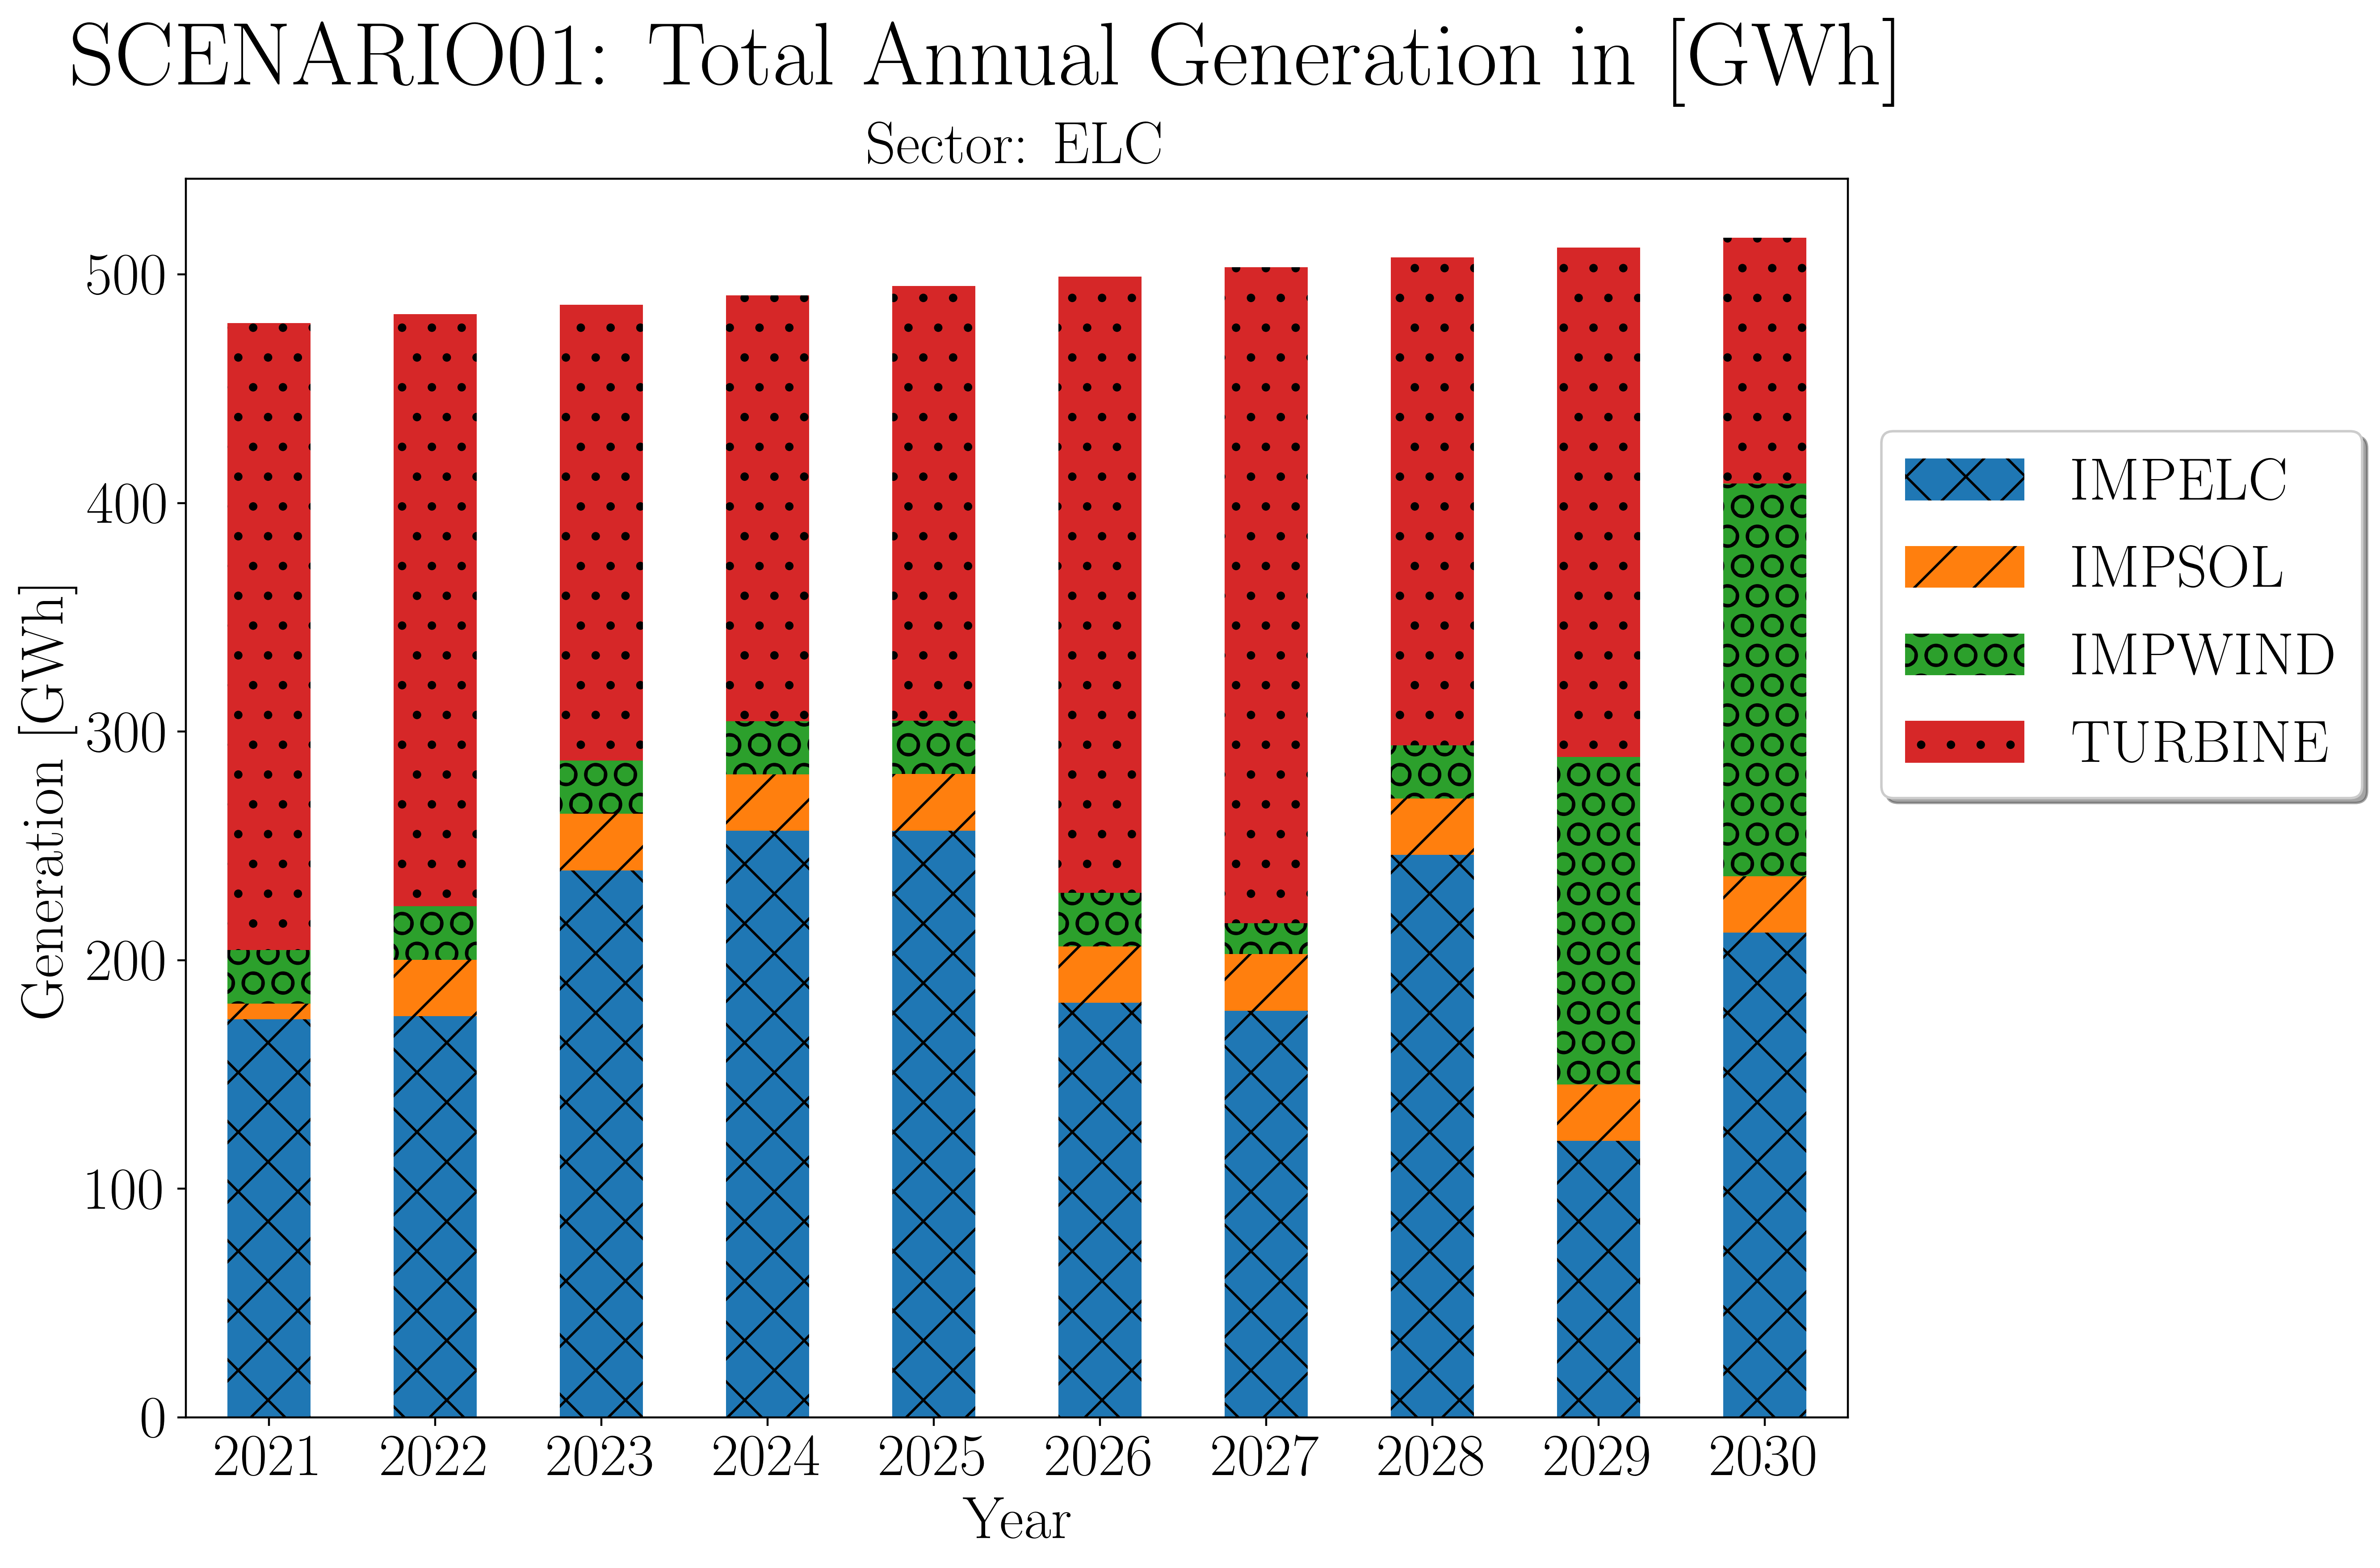
\includegraphics[width=\columnwidth]{scenario01_elc_generation.png}
	\caption{The projected breakdown of electricity generation in GWh(e), by
	source, for the next 10 years if \gls{uiuc} could build nuclear reactors at
	no cost.}
	\label{fig:s01_elc_gen}
\end{figure}

Since \gls{uiuc} is still importing electricity in this scenario the projected
carbon will not drop to zero. Figure \ref{fig:s01_all_co2} shows that the campus
emissions track exactly with the increase or decrease in imported electricity.

\begin{figure}[ht!]
	\centering
	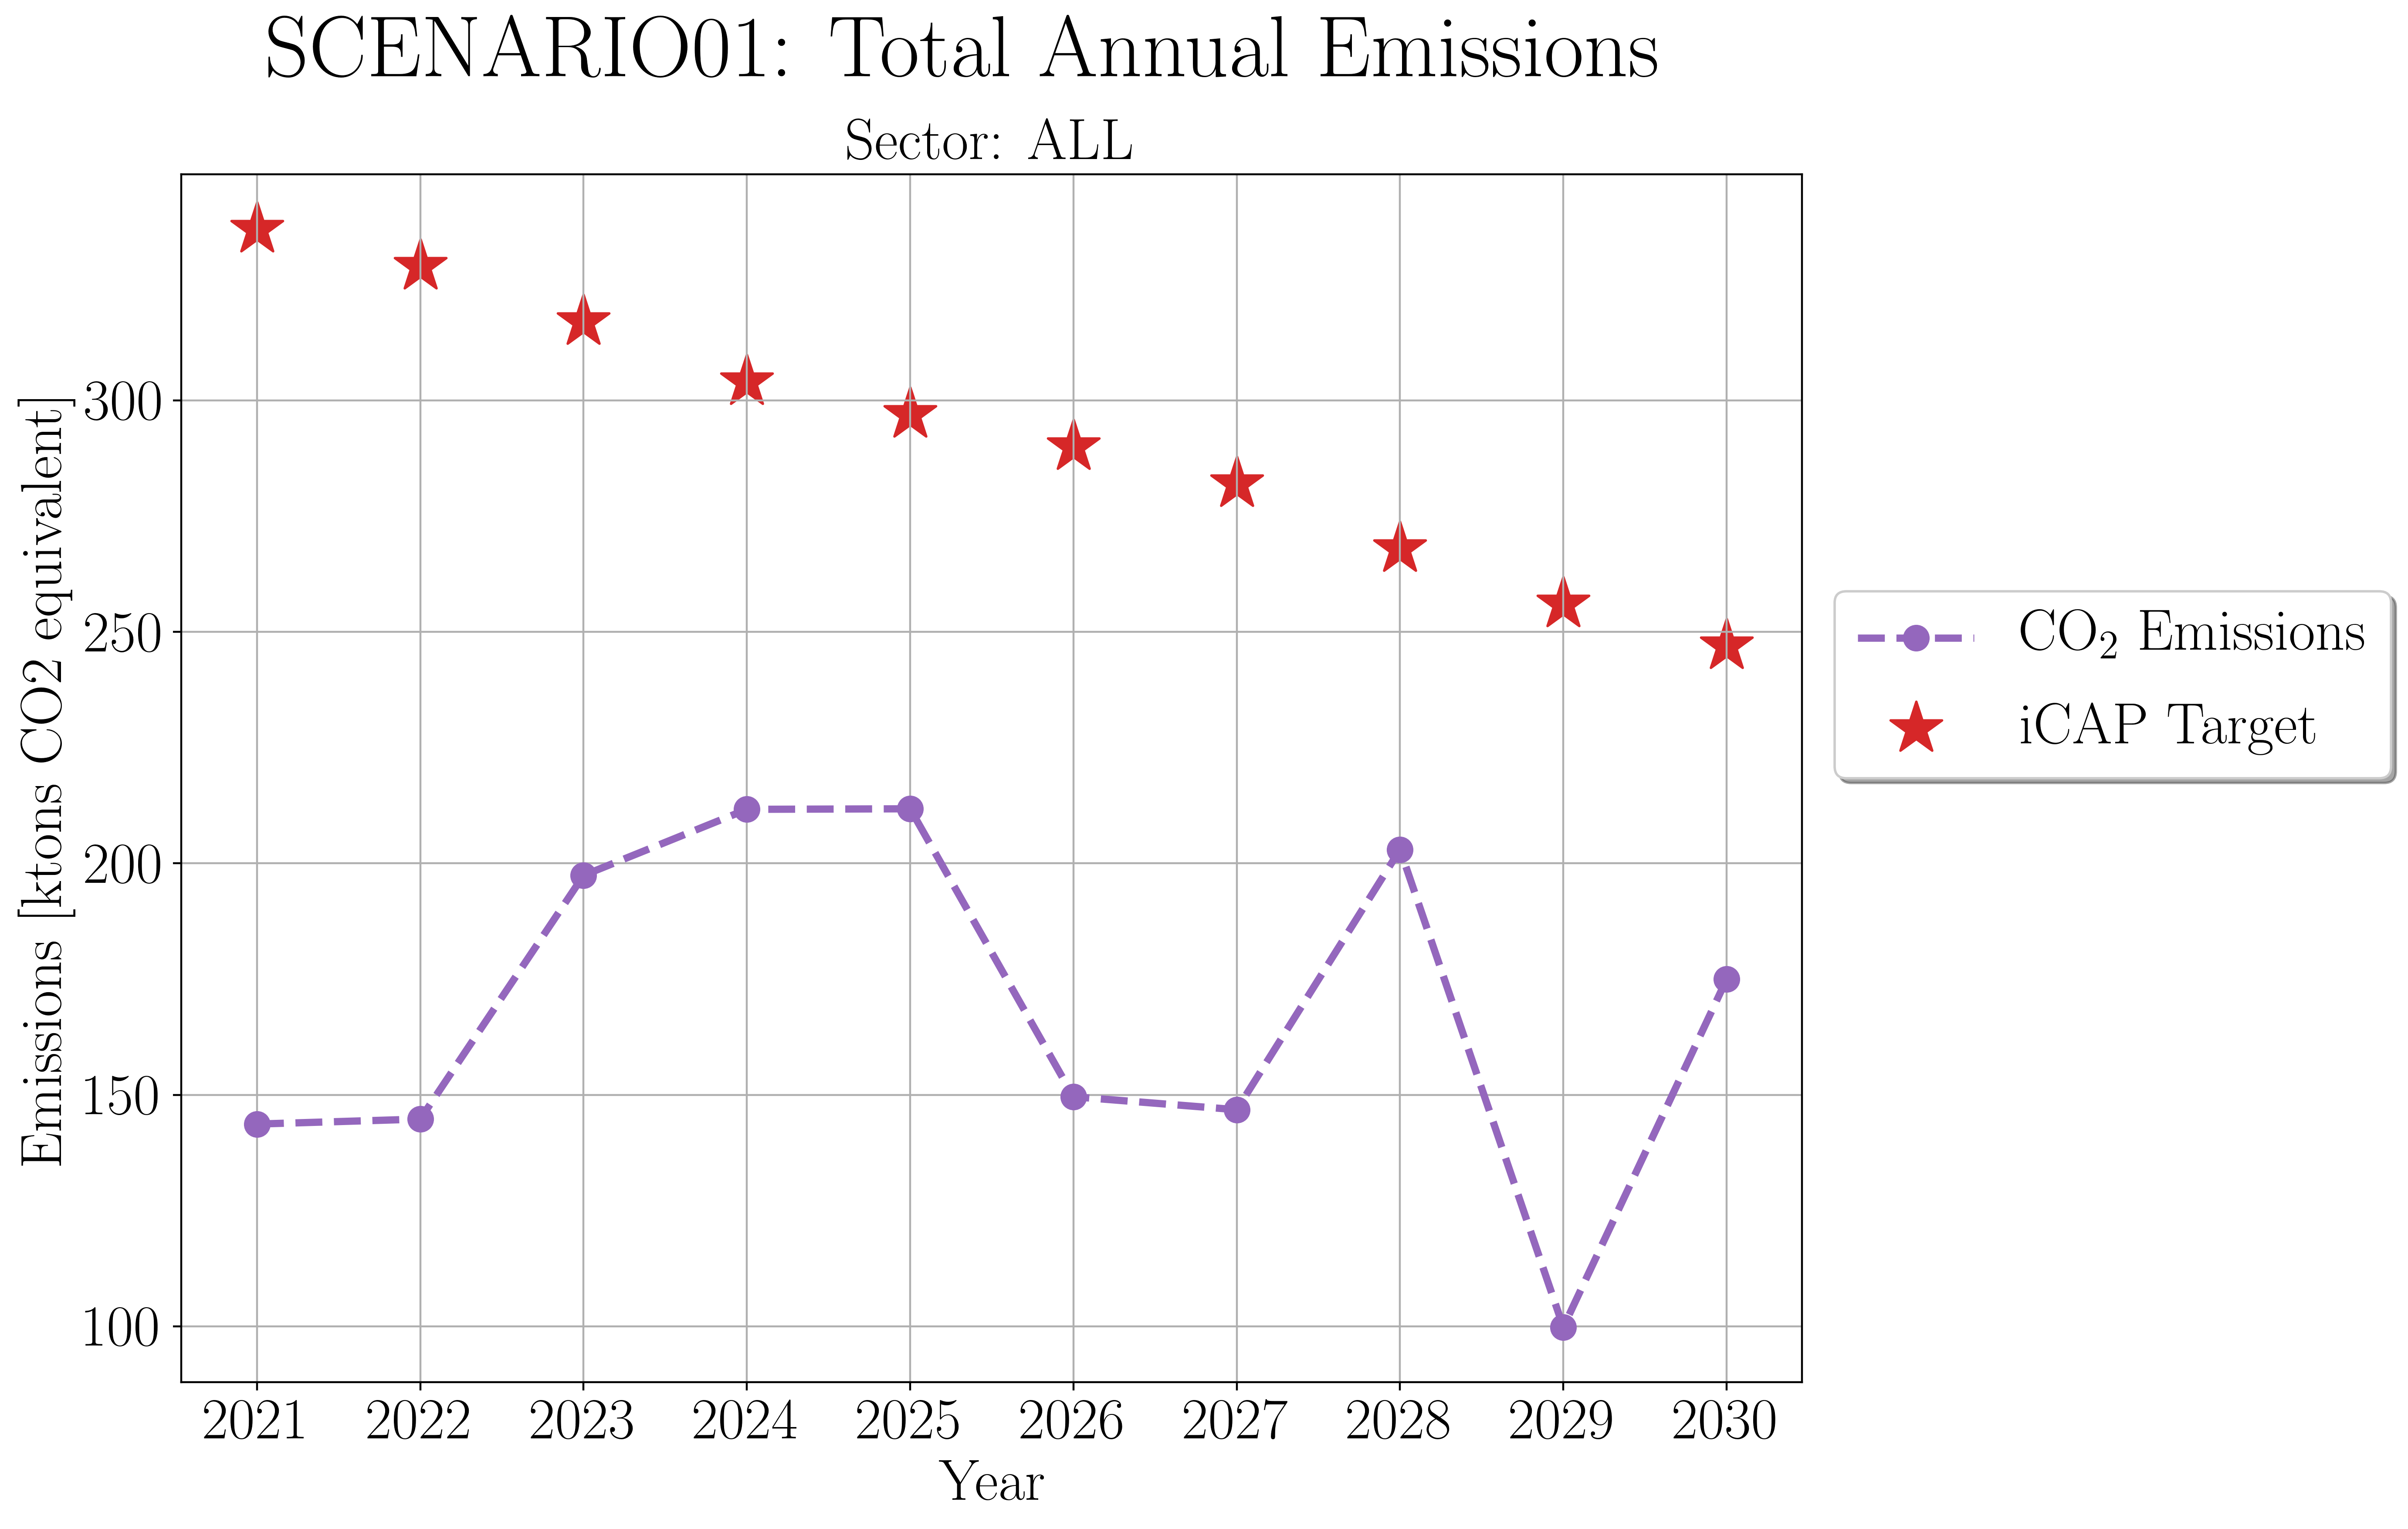
\includegraphics[width=\columnwidth]{scenario01_all_emissions.png}
	\caption{The Temoa projected carbon emissions for the next 10 years if
	\gls{uiuc} could build nuclear reactors at no cost.}
	\label{fig:s01_all_co2}
\end{figure}


\subsection{Scenario 2: Nuclear Reactors With Capital Cost}

The second scenario is somewhat more realistic because building a reactor
includes a capital cost, however, the total capacity is still unconstrained.
As in Scenario 1, Figure \ref{fig:s02_ind_cap} and Figure \ref{fig:s02_ind_gen}
show that \gls{app} is quickly replaced by nuclear capacity. However, Temoa
used \gls{app} in the first year due to the relatively high carbon allowance in
the first year and the capital costs of a nuclear power plant.

\begin{figure}[ht!]
	\centering
	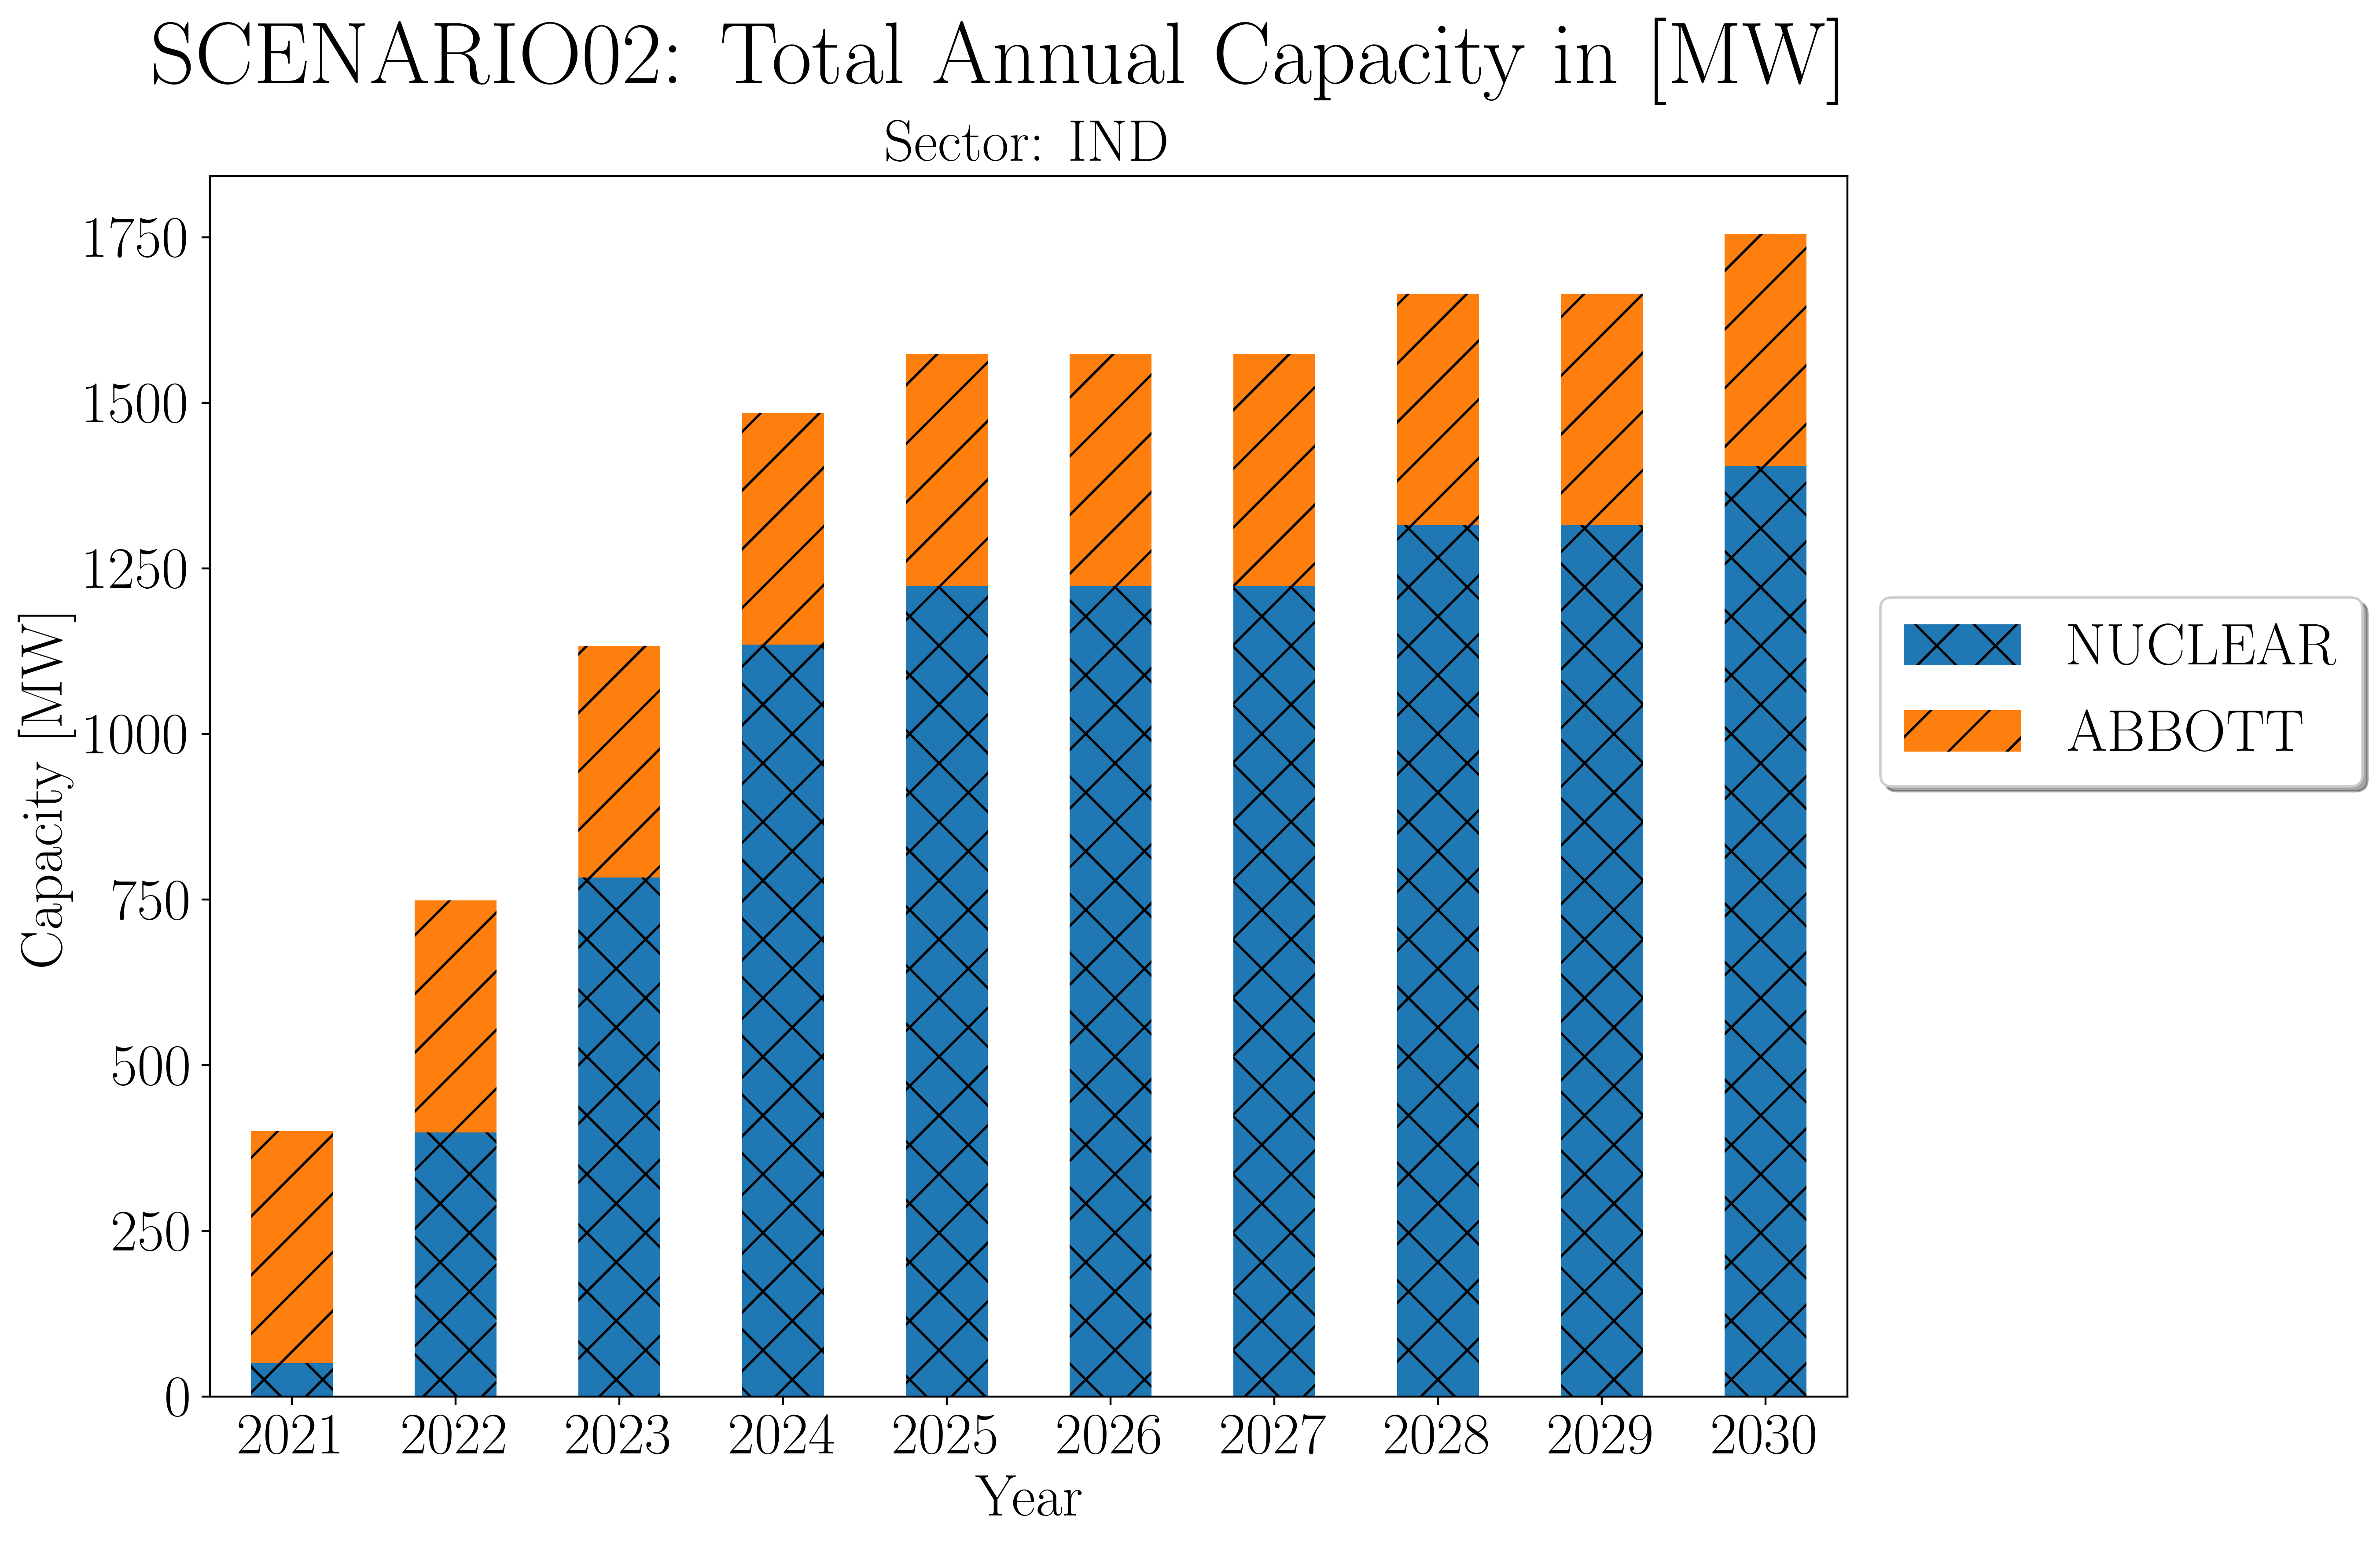
\includegraphics[width=\columnwidth]{scenario02_ind_capacity.png}
	\caption{The projected steam capacity in MW$_{th}$ for the next 10 years
	if \gls{uiuc} could build nuclear reactors at no cost.}
	\label{fig:s02_ind_cap}
\end{figure}

\begin{figure}[ht!]
	\centering
	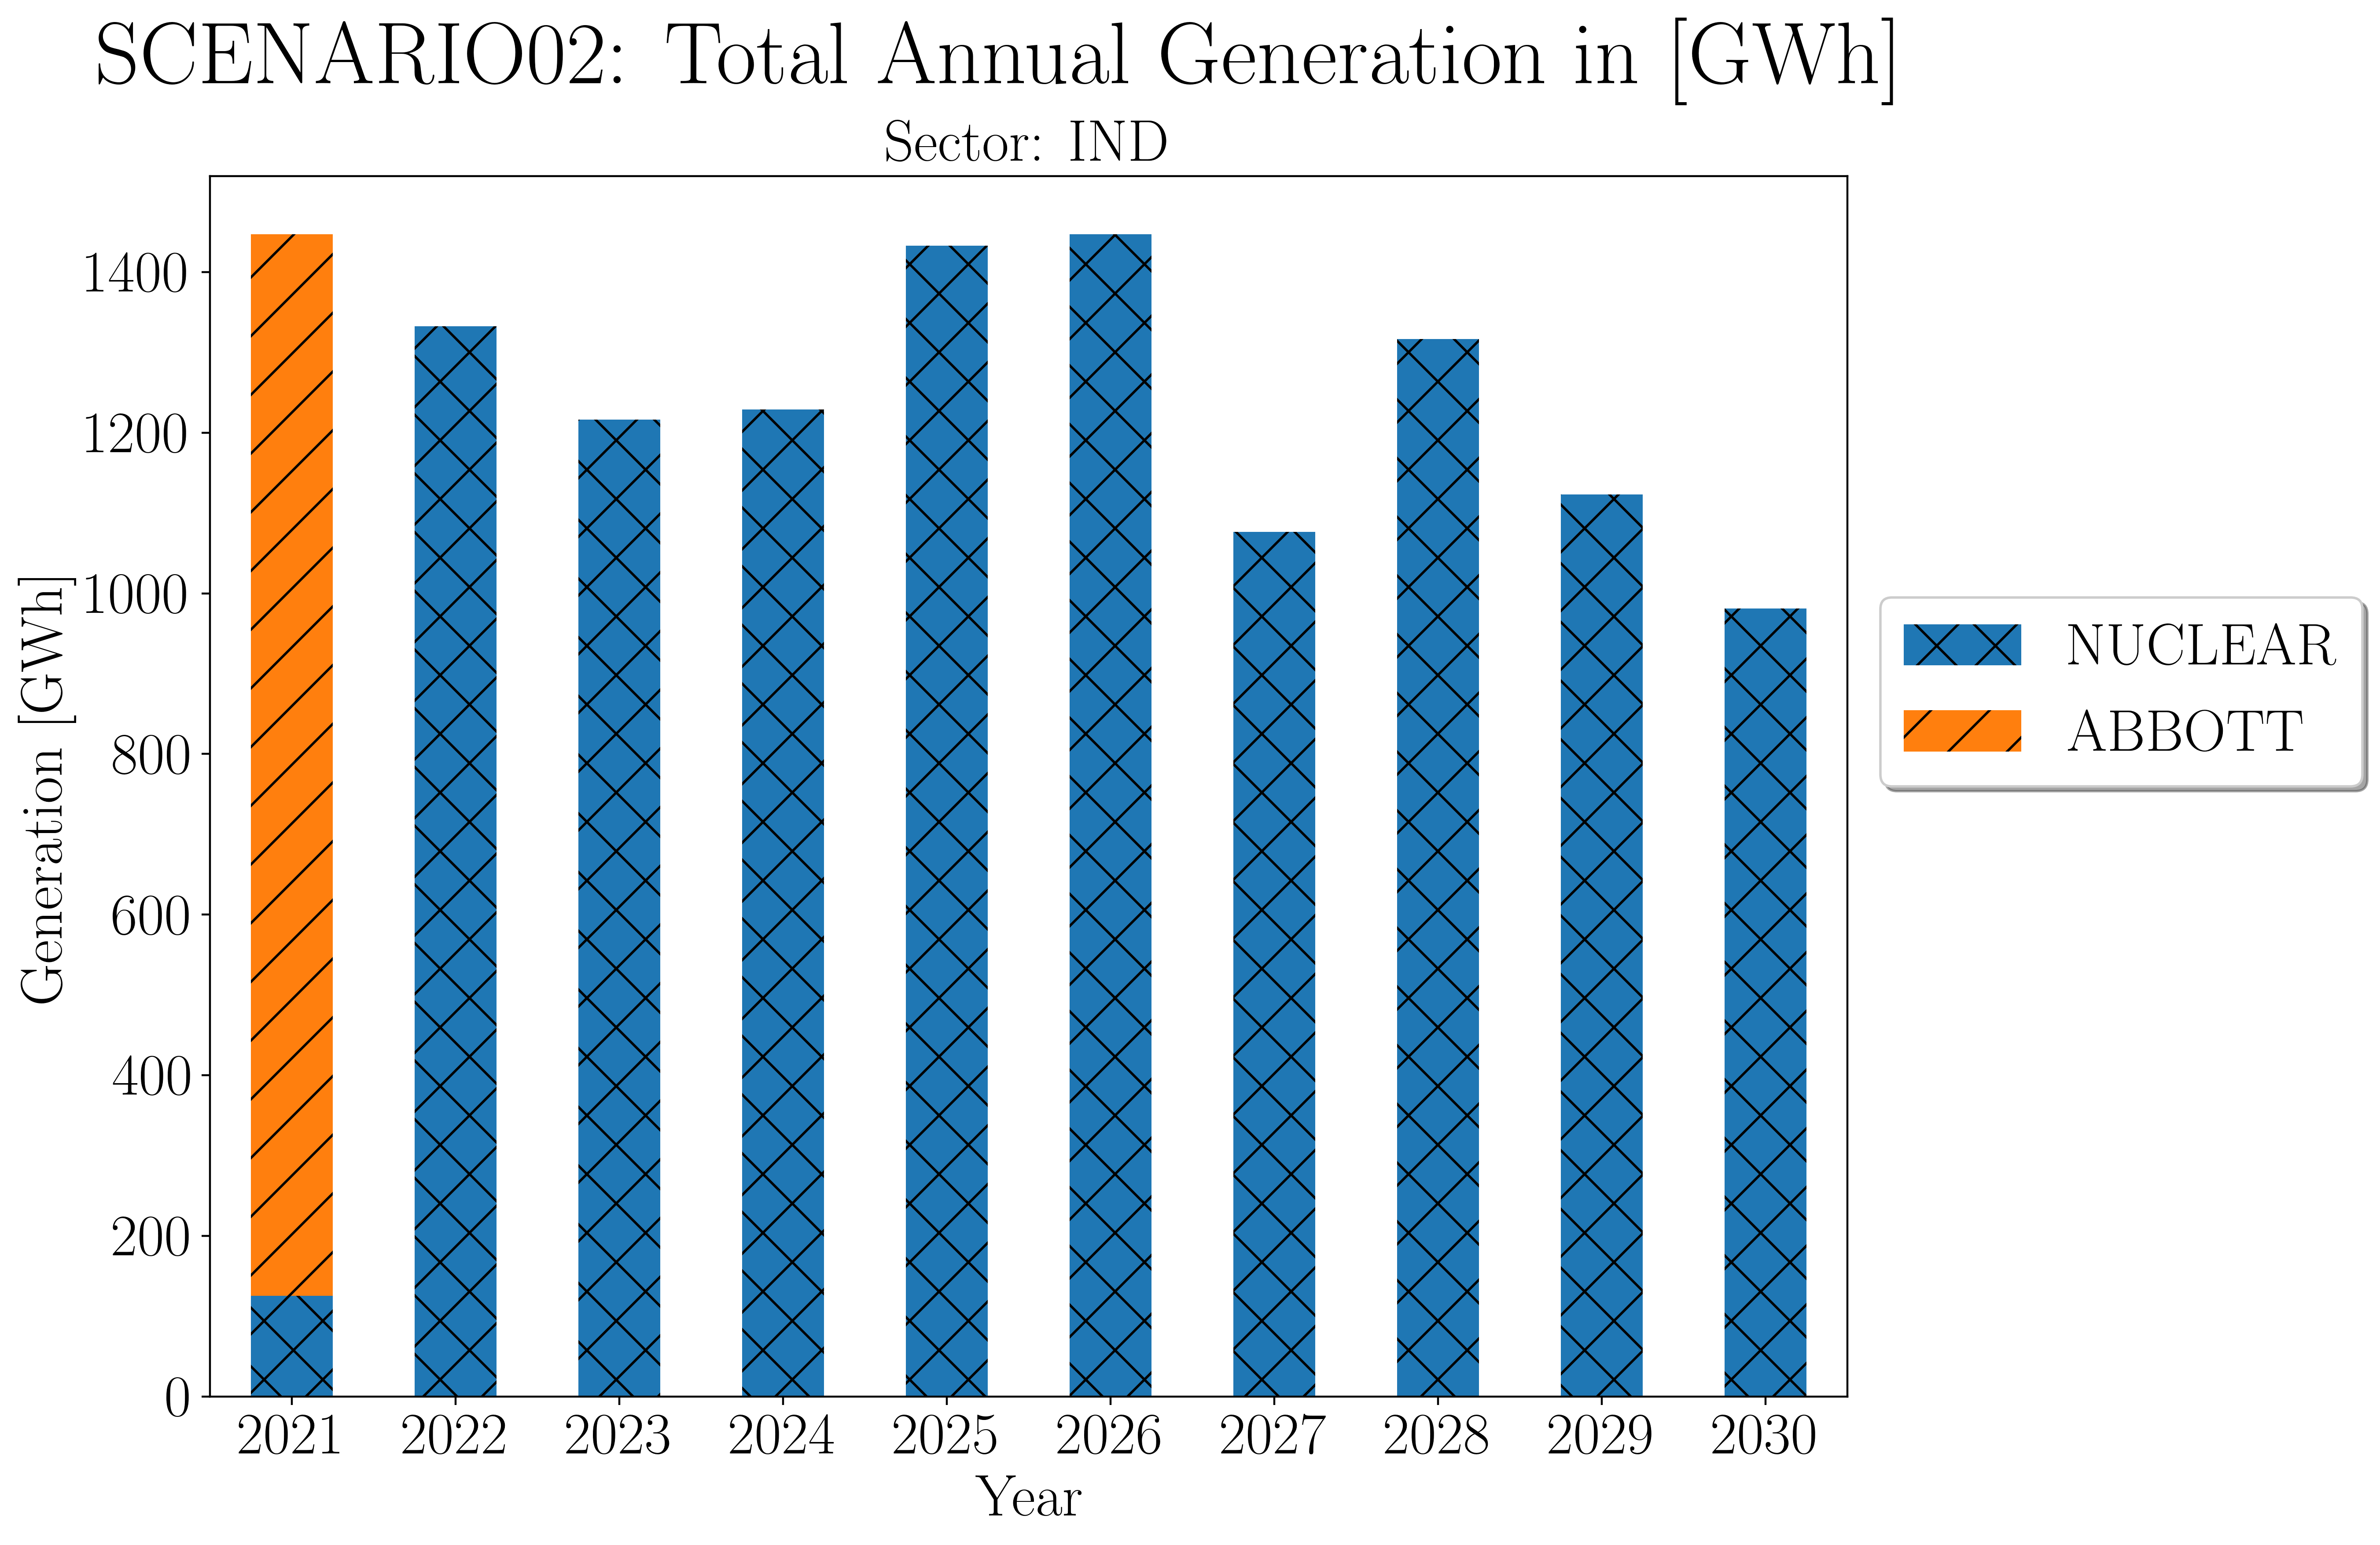
\includegraphics[width=\columnwidth]{scenario02_ind_generation.png}
	\caption{The projected breakdown of steam generation by source in GWh(th)
	for the next 10 years if \gls{uiuc} could build nuclear reactors at no cost.}
	\label{fig:s02_ind_gen}
\end{figure}

Similar to the results in Scenario 1, Temoa will use the flexibility, or lack
thereof, in the carbon limits to determine the lowest cost solution. Since some
carbon emissions are allowed, the most cost effective approach is to use
imported electricity as shown in Figure \ref{fig:s02_elc_gen}. In addition to
electricity imports, Figure \ref{fig:s02_elc_cap} shows \gls{uiuc} expanding
it's wind \gls{ppa} after the current one expires in 2026
\cite{breitweiser_wind_2016}.

\begin{figure}[ht!]
	\centering
	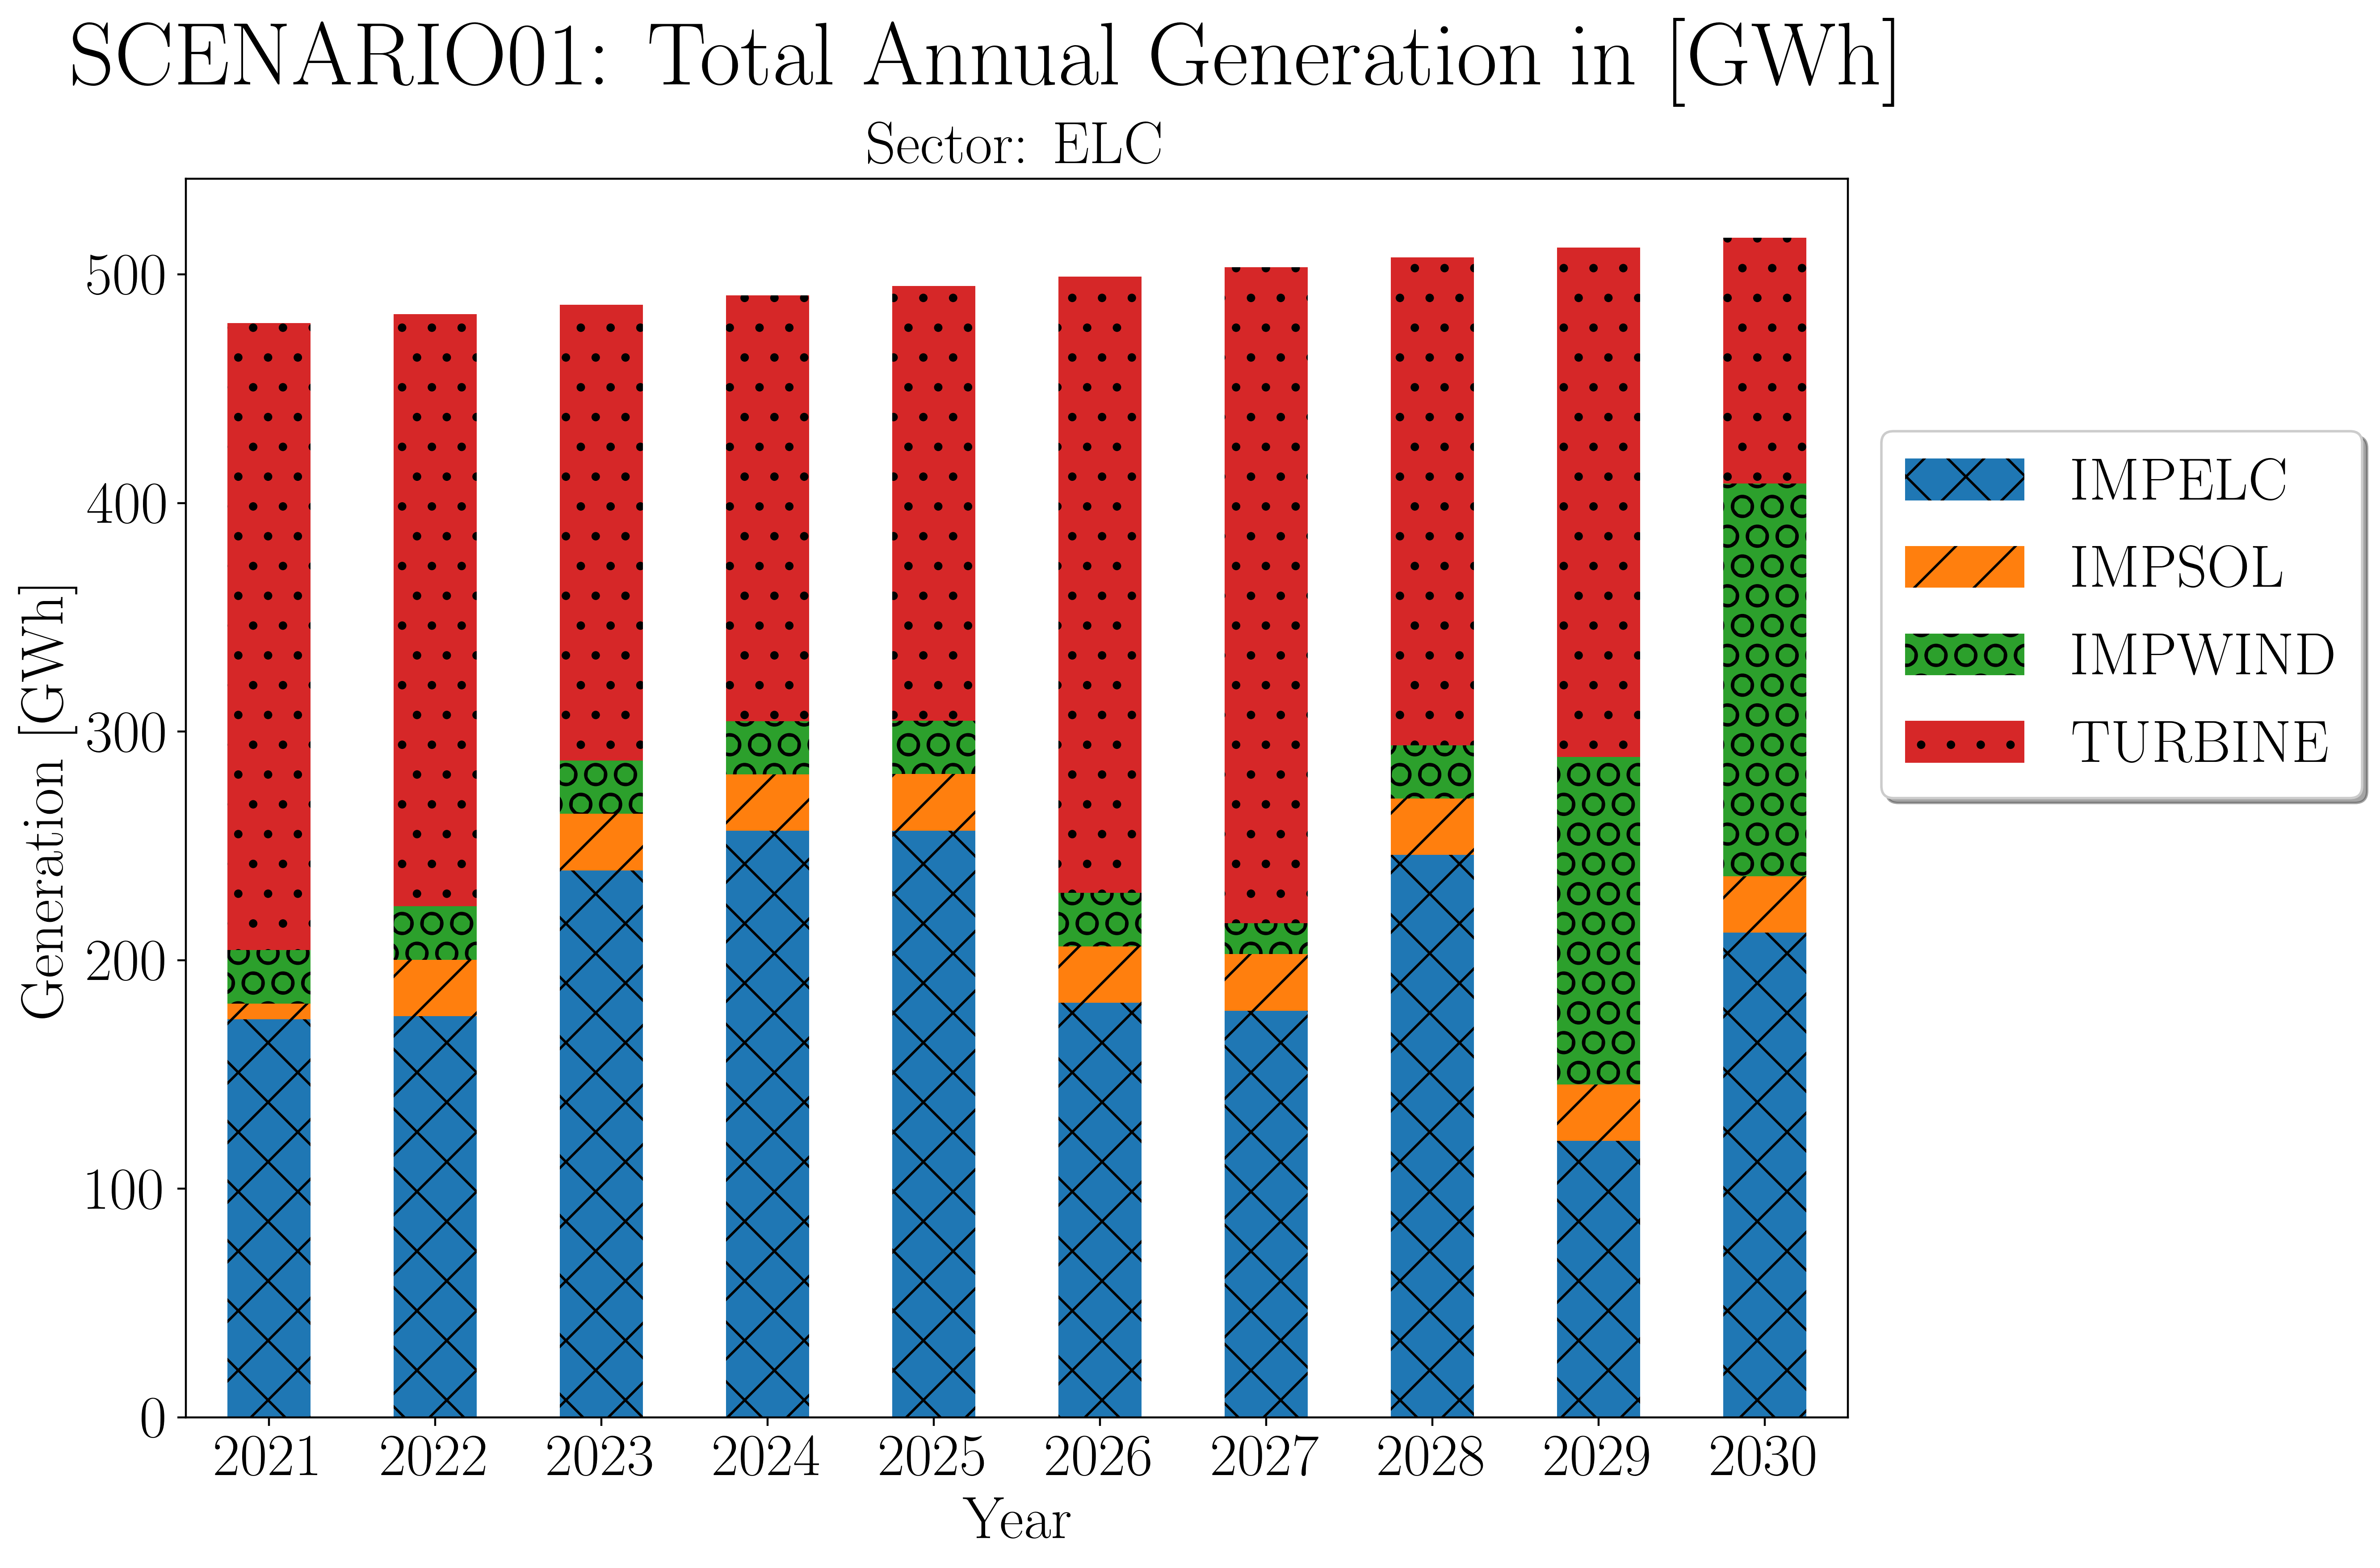
\includegraphics[width=\columnwidth]{scenario01_elc_generation.png}
	\caption{The projected breakdown of electricity generation in GWh(e), by
	source, for the next 10 years at
	\gls{uiuc}.}
	\label{fig:s02_elc_gen}
\end{figure}

Increasing the amount of electricity purchased
from a wind farm is cheaper than building more nuclear capacity because the
reactor is responsible for steam demand, while electricity demand can be met
through other means. In this scenario, the wind \gls{ppa} grows to a capacity of
100.5 MW$_e$, which is the entire installed capacity of Rail Splitter Wind Farm
\cite{breitweiser_wind_2016}.

\begin{figure}[ht!]
	\centering
	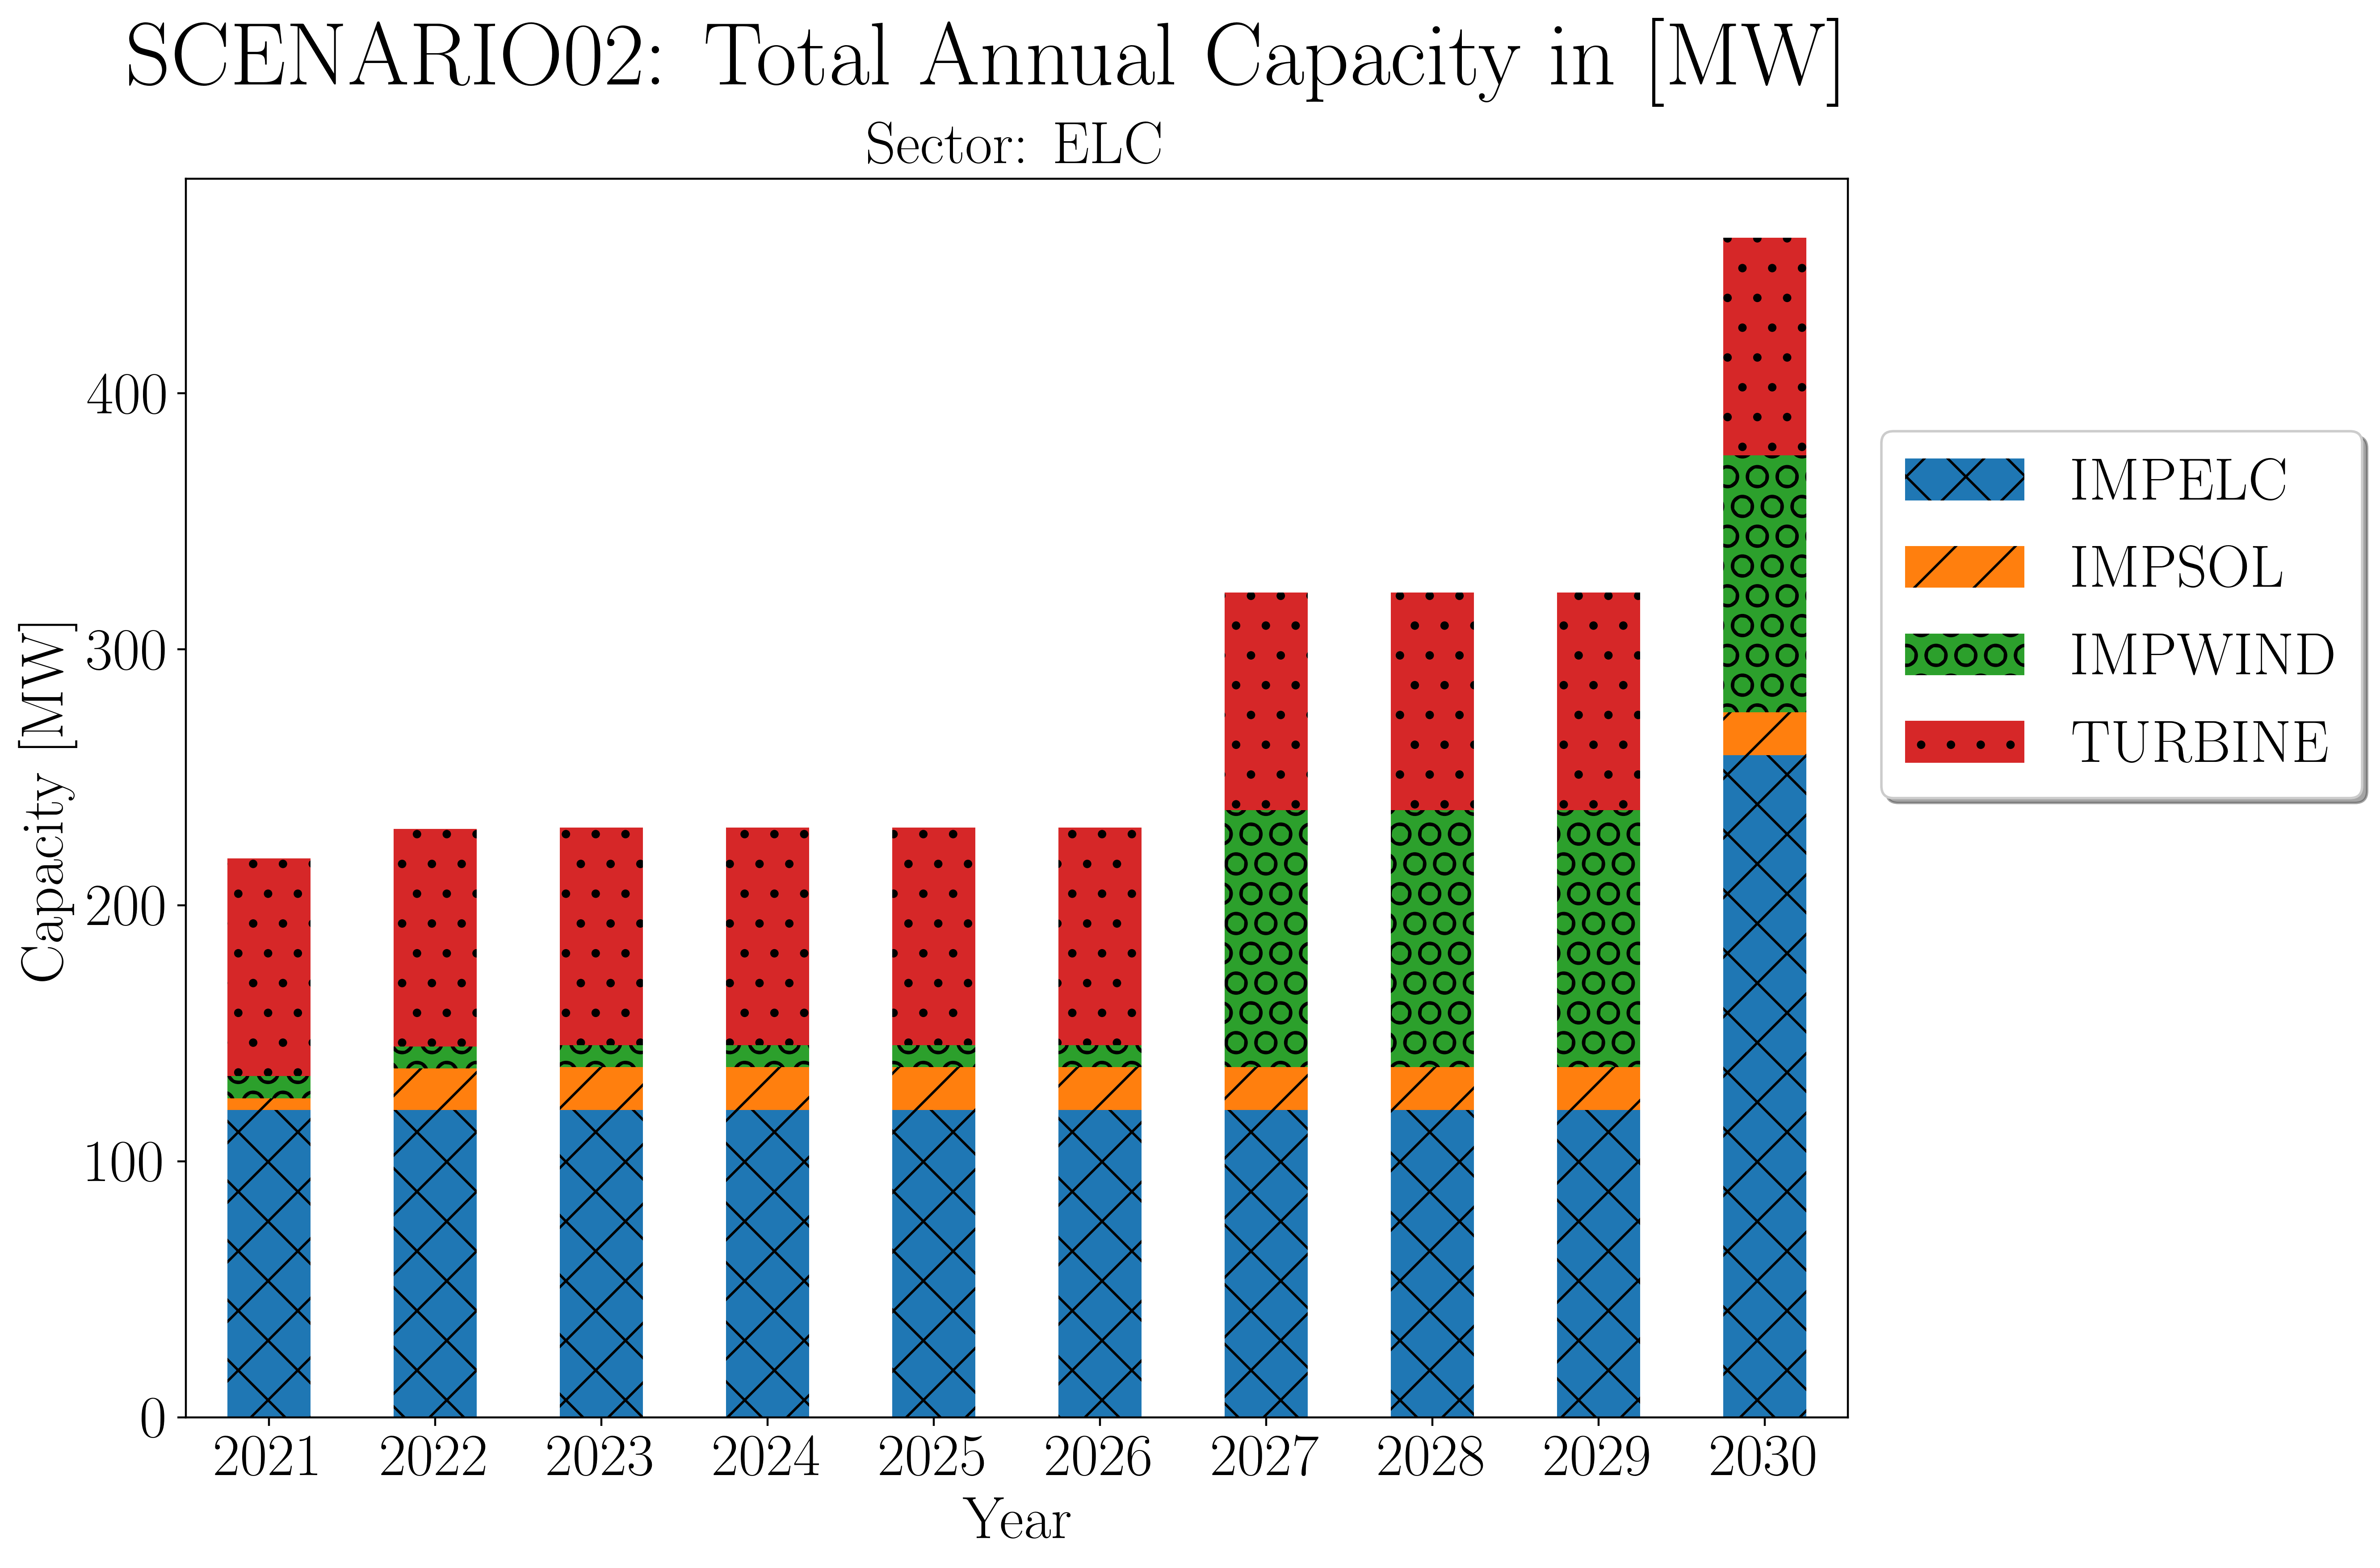
\includegraphics[width=\columnwidth]{scenario02_elc_capacity.png}
	\caption{The projected electric capacity in MW$_{e}$ for the next 10 years at
	\gls{uiuc}.}
	\label{fig:s02_elc_cap}
\end{figure}

The carbon emissions in this scenario, shown in Figure \ref{fig:s02_all_co2},
also follow a similar trend to Scenario 1. The key difference is in the first
year when \gls{app} is still being used to produce steam and electricity.

\begin{figure}[ht!]
	\centering
	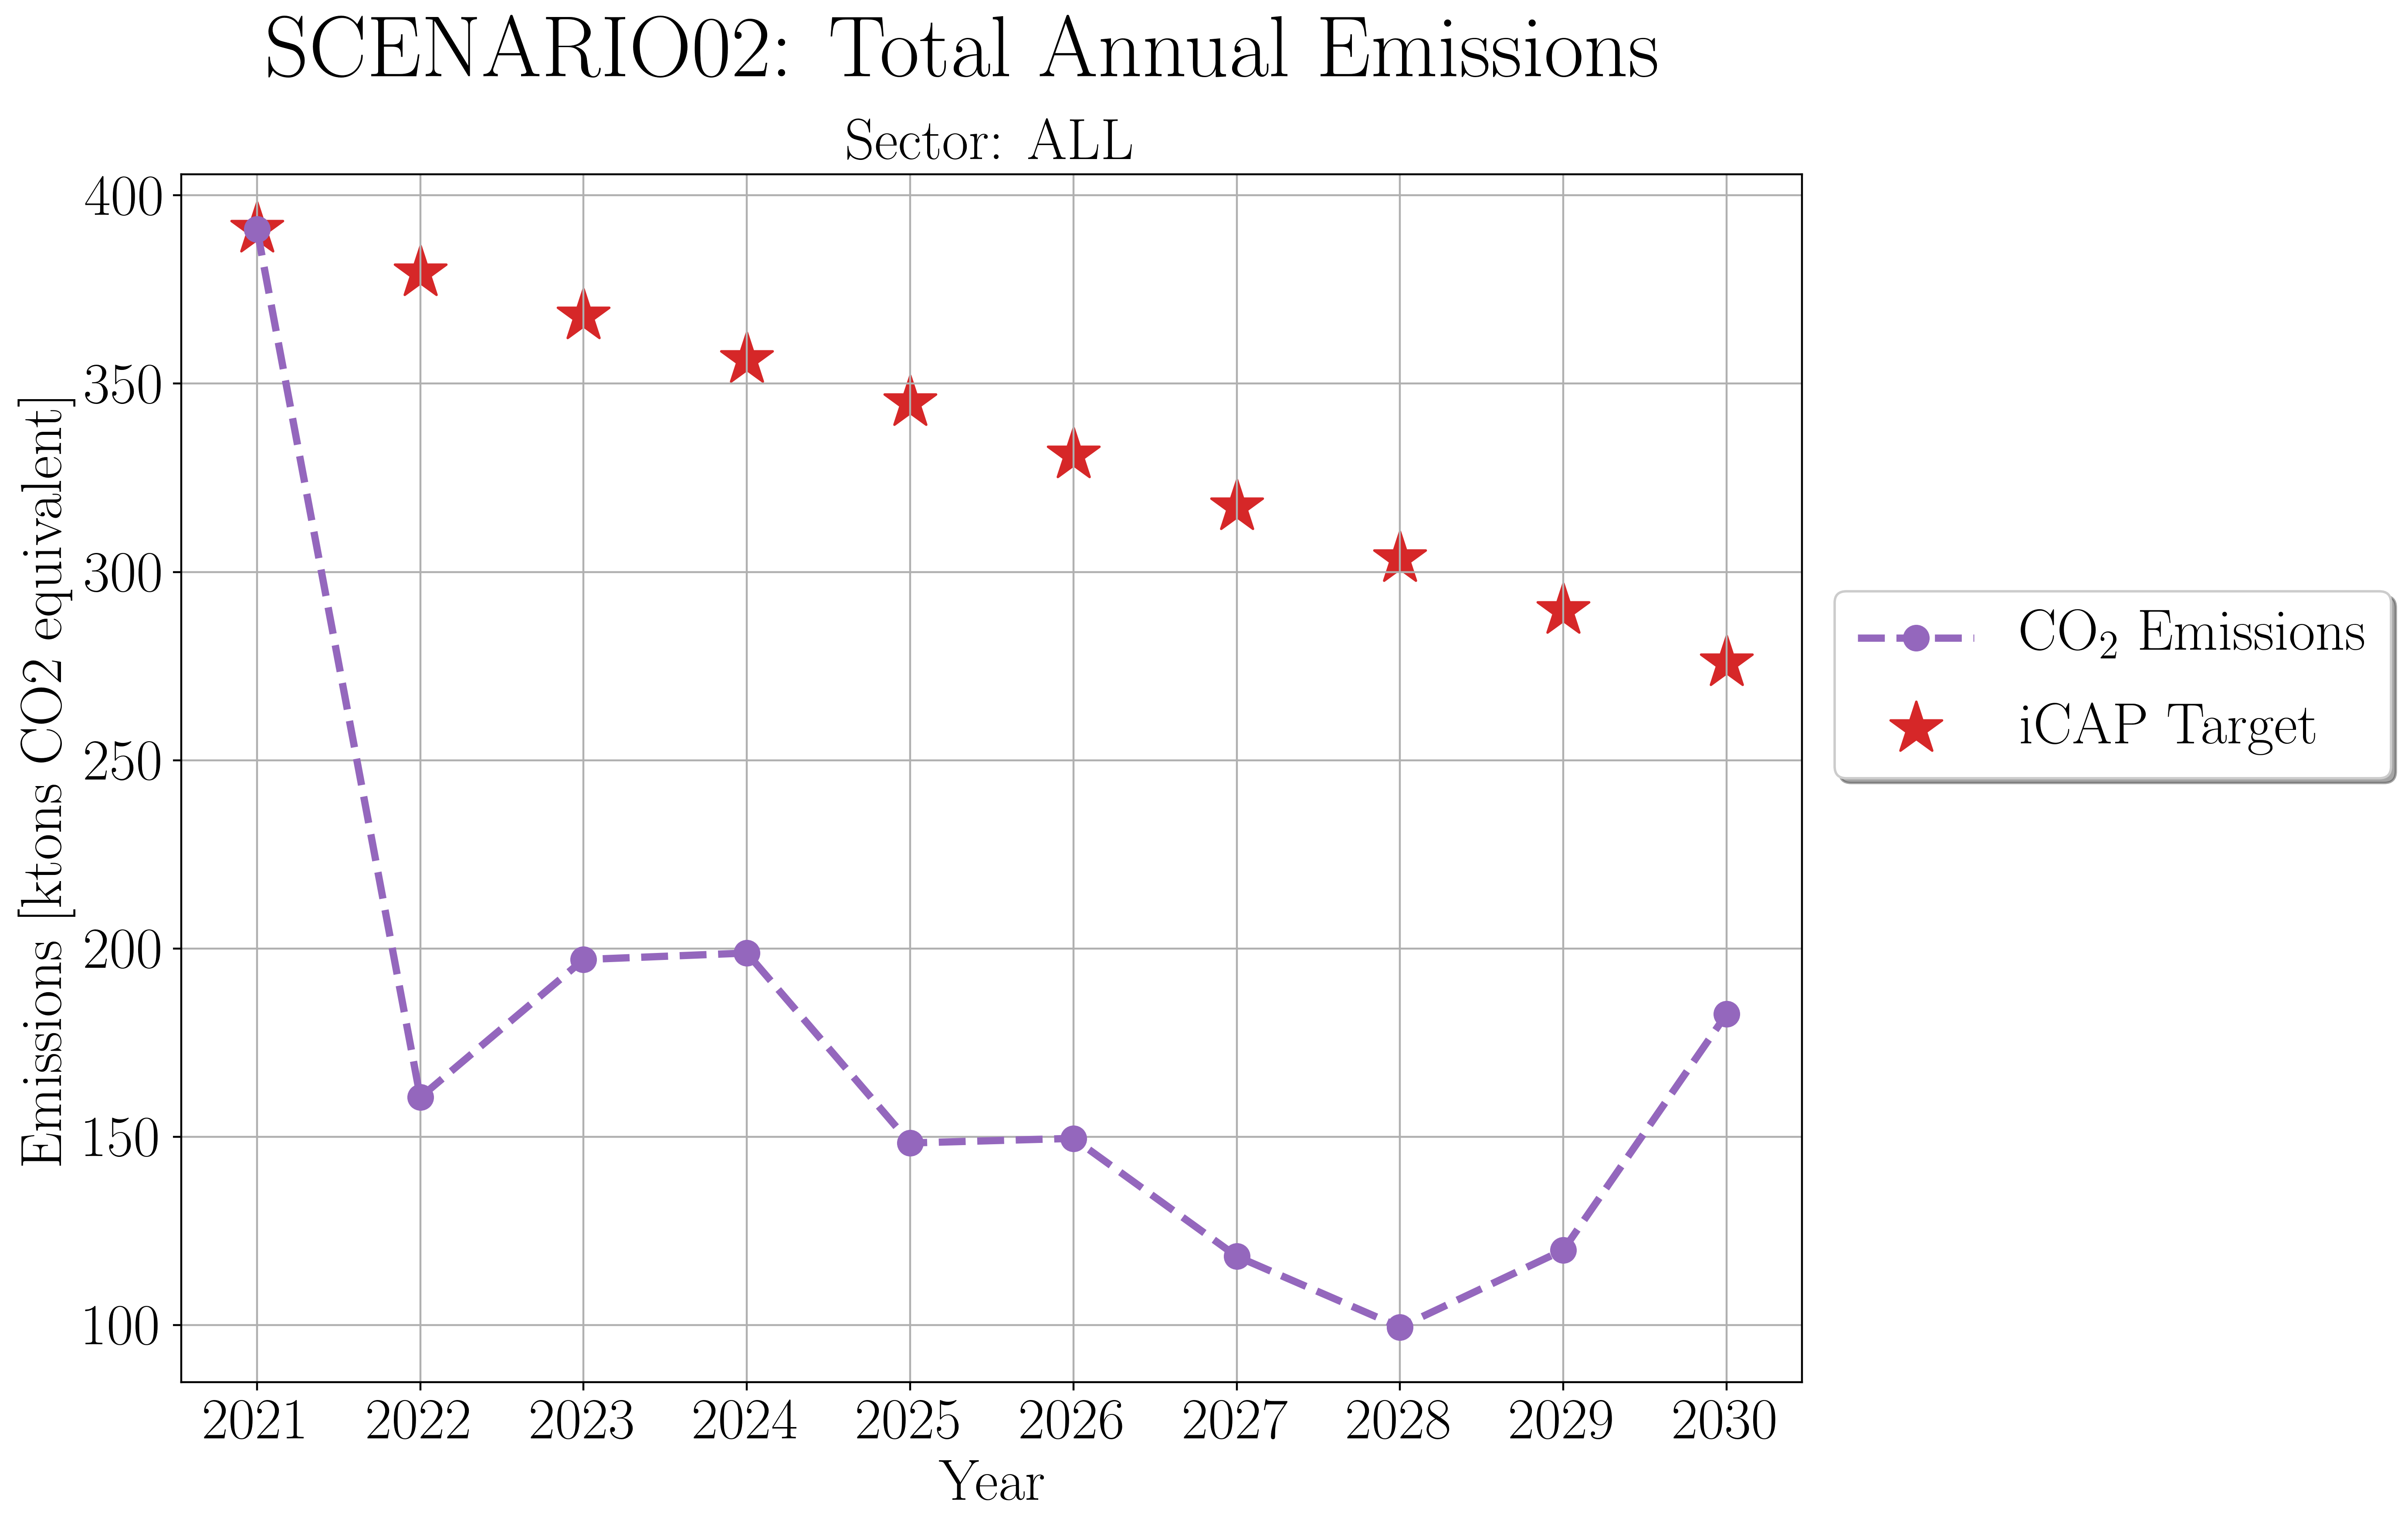
\includegraphics[width=\columnwidth]{scenario02_all_emissions.png}
	\caption{The carbon emissions projected by Temoa for the next 10 years at
	\gls{uiuc}.}
	\label{fig:s02_all_co2}
\end{figure}
These results show that \gls{uiuc}'s carbon goals can be initially met with a
slower introduction of nuclear power.


\subsection{Scenario 3: Small Modular Reactor}
The final scenario limited the capacity of a nuclear reactor to 100  MW$_th$
for a \gls{smr}. Due to physical size constraints a nuclear reactor
for power production on a university campus will most likely be an \gls{smr}.
Figure \ref{fig:s03_ind_cap} shows that an \gls{smr} is not large enough
to replace \gls{app} but a reactor with a rated capacity less than 100 MW$_th$
can still help \gls{uiuc} satisfy the carbon goals outlined in \gls{icap}.

\begin{figure}[ht!]
	\centering
	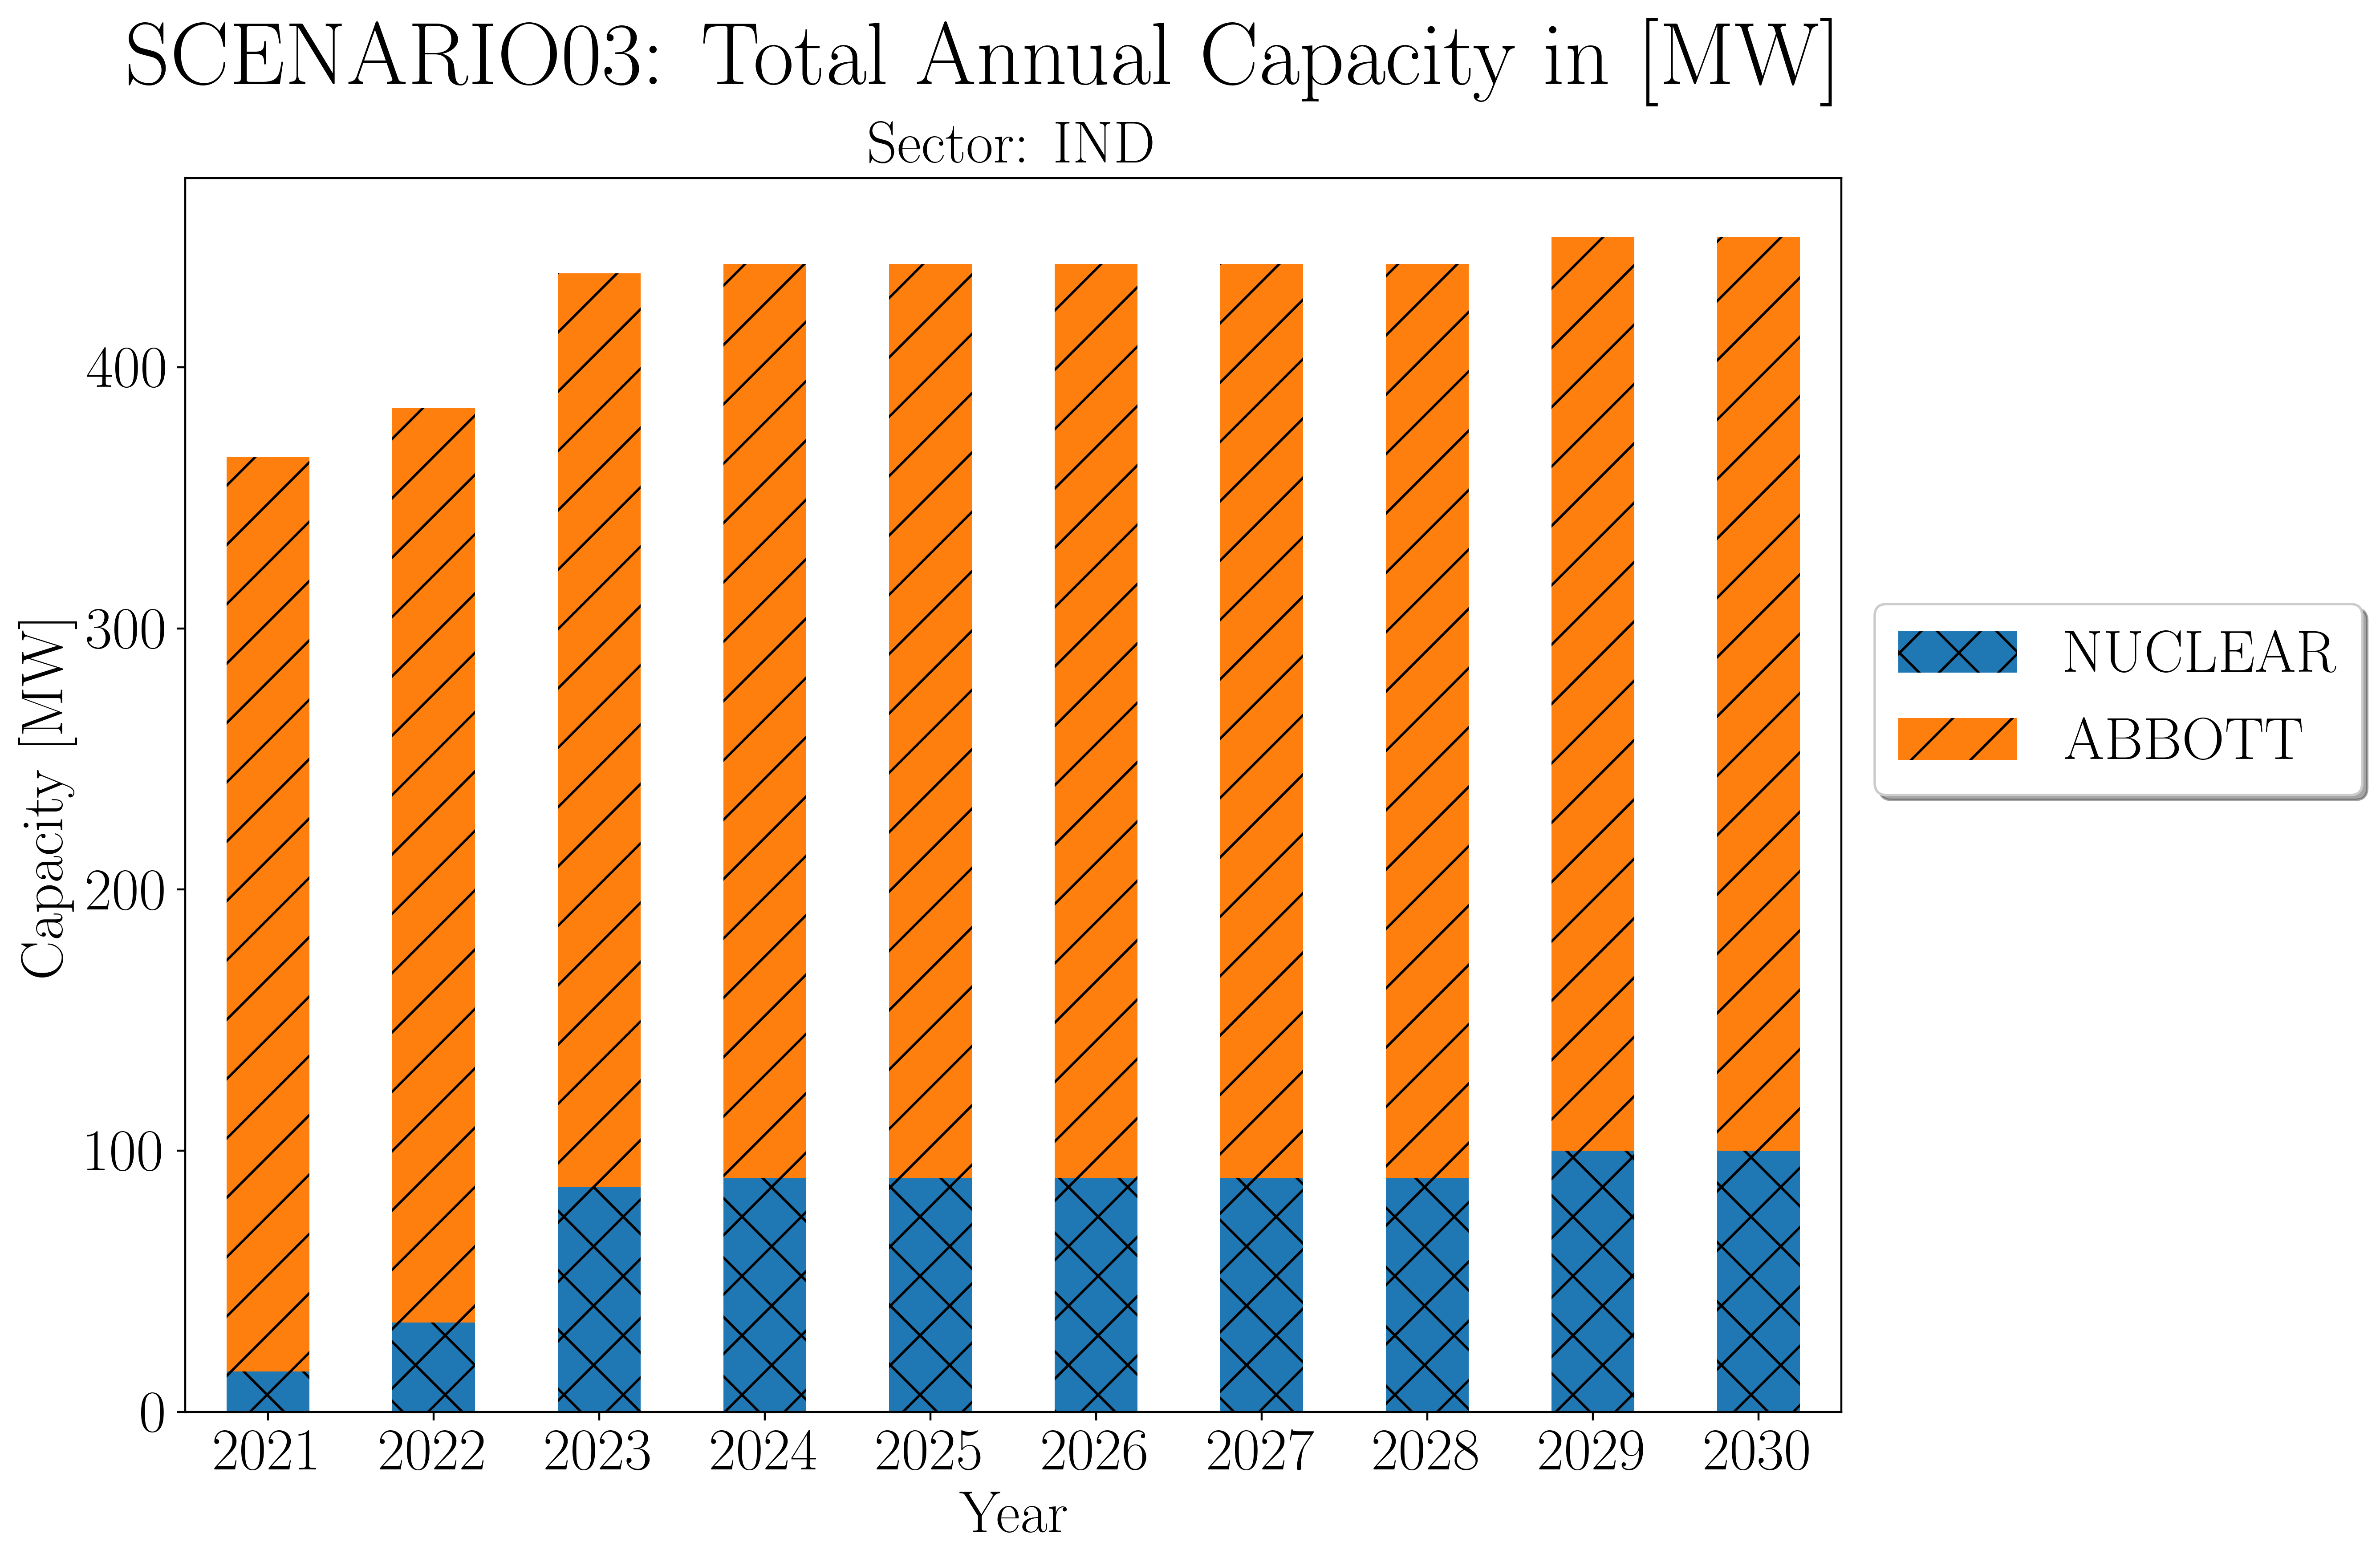
\includegraphics[width=\columnwidth]{scenario03_ind_capacity.png}
	\caption{The projected steam capacity in MW$_{th}$ for the next 10 years if
	\gls{uiuc} invests in \glspl{smr}.}
	\label{fig:s03_ind_cap}
\end{figure}
